
\chapter{Grafisches Design}\label{ch:grafikdesign}

\renewcommand{\kapitelautor}{Autor: Markus Böheim}

\section{Grafische Tools/Programme}

Für ein Projekt dieser Größe
ist ein einheitliches Design und eine konsistente Arbeitsweise wichtig, um das gewünschte Ergebnis zu erzielen.
Die Programme, die verwendet werden, um alle Grafiken und Assets zu erstellen, spielen daher eine große Rolle.
Die HTL Rennweg ermöglicht Schülerinnen und Schülern einen Zugang zu der Adobe Creative Cloud Suite, welche die gr
ößten und wichtigsten Design-Programme zur Verfügung stellt. Da das Diplomarbeitsteam bereits in den letzten vier Jahren der HTL einigermaßen Erfahrung mit der Adobe Creative Cloud gesammelt hat, ist diese und ihre Programme die richtige Wahl für \FF.

\subsection{Adobe XD}

Adobe Xd ist ein Programm, welches für das Designen von User Interfaces, Wireframes und Applikationen von Adobe
entwickelt und 2015 veröffentlicht wurde. \zit{adobeXD} Adobe Xd erlaubt es einem, schnell Designs auf Zeichenfl
ächen zu
erstellen,
die anschließend mit der \quoted{Prototyp} Funktion miteinander verknüpft und interagierbar gemacht werden.
Da dieses Programm teil der Adobe Creative Cloud ist, lässt es sich sehr einfach mit Adobe Photoshop und Illustrator nutzen, welche unter anderem verwendet wurden, um die Assets und Grafiken für \FF zu erstellen. Ein weiterer
\quoted{Selling-Point}
für das UI/UX Programm von Adobe, ist die Echtzeit Co-Editing Funktion, welche es dem Team ermöglicht, gleichzeitig an dem Mock Up von \FF zu arbeiten ohne Verzögerungen oder Einsatz eines Versionierungssystems.
Für \FF wurde Adobe Xd hauptsächlich für das Gestalten des Game User Interfaces verwendet, als auch für die Webseite
, sowie sämtliche Grafiken für Steam, Plakate oder Social Media Posts, da es ein vektorbasiertes Programm ist. Andere
Programme wie Adobe Photoshop oder Illustrator wären auch gut geeignet für alle Grafiken außerhalb des Spiels,
besitzen allerdings keine Echtzeit Co-Editing Funktion und sind daher nicht die optimale Wahl für den Zweck der
Diplomarbeit \zit{coEdit}.

\subsection{Adobe Photoshop}

Adobe Photoshop ist ein Bildbearbeitungsprogramm für Rastergrafiken des Herstellers Adobe. Das Programm ist
heutzutage ein Industriestandard und der weltweite Marktführer in der Design Branche und wird von Fotografen,
Künstlern und Grafikdesignern verwendet. Adobe Photoshop ist Teil der Adobe Creative Cloud und stellt daher eine gute
Verbindung zu den anderen Programmen der Creative Cloud wie Illustrator oder Premiere Pro her. Tools wie Masken,
Auswahlwerkzeuge, Zeichenwerkzeuge und komplexe Filter ermöglichen es einem, jeden kreativen Gedanken beim Erstellen
des \FF Mockups umzusetzen, wie beispielsweise Hintergründe, Buttons, User Interface Elemente oder Icons. \zit{
    photoshop}
Für \FF ist die Kombination von Photoshop und Adobe Xd besonders praktisch, da die Funktion
\quoted{in Photoshop bearbeiten} in Adobe Xd,
Photoshop öffnet und direkte Veränderungen an dem ausgewählten Bild in Xd übertragen kann. Dadurch erspart man sich das langwierige, mehrmalige Exportieren von Assets, die jedes Mal neu in eine Zeichenfläche eingefügt werden müssten.
Mit Pinseln ist es möglich sich vielseitig auszudrücken beim Erstellen von Assets für Videospiele. Mit Pinselsets ist es möglich, den Stil von verschiedenen Werkzeugen wie Öl Pinsel, Tinte oder einen Bleistift zu replizieren. Adobe Photoshop bietet ein vorinstalliertes Pinselset von Kyle T. Webster an, welches in \FF verwendet wurde, um Icons wie zum Beispiel das Kampf-Symbol zu erstellen.

\begin{figure}[H]
    \centering
    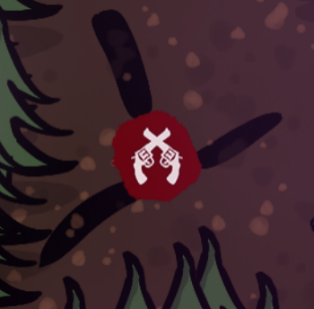
\includegraphics[width=0.4\textwidth]{kampfSymbol.png}
    \caption{Kampf Symbol auf der Map}
\end{figure}

Dieses Pinselset beinhaltet 20 verschiedene Pinsel, wobei hauptsächlich \quoted{Klassischer Cartoonist} verwendet
wurde. Mit diesem Pinsel ist es einfach Tinte zu replizieren, was bei \FF hilft, den wilden Westen Stil zu verpassen
. Unter anderem wurde auch ein zweites Pinselset von ArtistMef verwendet, welches lizenzfrei ist und eine Vielfalt an
Pinseln bietet \zit{inkBrushes}. Beispielsweise wurde die Form eines Buttons des Statistik Bildschirmes zuerst mit dem
\quoted{Sketching Brush} Pinsel erstellt und anschließend mit dem \quoted{Spray Brush} Pinsel texturiert, um Tiefe und Detail in den Button zu bringen.

\begin{figure}[H]
    \centering
    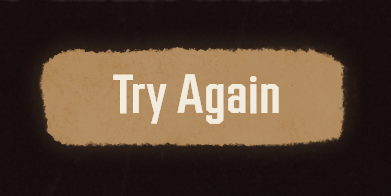
\includegraphics[width=0.4\textwidth]{tryAgainButton.png}
    \caption{\quoted{Try Again} Button im Statistik Fenster}
\end{figure}

Diese Pinsel können jeweils noch weiterhin angepasst werden unter den Pinseleinstellungen mit Optionen wie der Streuung, die bestimmt, wie breit der Pinsel aufgetragen wird oder Einstellungen zur Struktur des Pinselauftrags selbst. Je nach Einstellungen ist es einem möglich, seinen Assets einen einzigartigen Look zu verpassen und ein passendes, einheitliches und wiedererkennbares Design zu kreieren.

\begin{figure}[H]
    \centering
    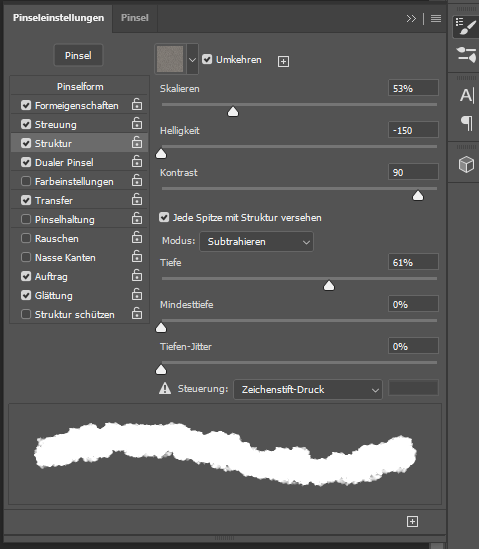
\includegraphics[width=0.4\textwidth]{pinselStruktur.png}
    \caption{Struktur Einstellungen eines Pinsels in Photoshop} 
\end{figure}

Eine weitere Methode um den Elementen von \FF den rustikalen western Look zu verpassen ist mit Texturing. Mit den
Mischmodi von Photoshop ist es möglich einem beliebigen Objekt beispielsweise eine papier-artige Textur zu geben,
indem eine weitere Ebene erstellt wird mit einem Bild von einem alten Stück Papier und einen passenden Mischmodus
auswählt. Der Mischmodus bestimmt, wie sich ein Mal- bzw. Bearbeitungswerkzeug auf die Pixel im Bild auswirkt \zit{
    mischmodi}. Zusätzlich kann mit einer Schnittmaske die Bildtextur auf die Pixel der darunterliegenden Ebene
zugeschnitten werden. Diese Technik wird bei jedem Asset, welches als Hintergrund für Pop-Up Fenster oder ähnlichen dient, angewendet.

\subsection{Adobe Illustrator}

Illustrator ist Adobes größtes vektorbasierte Computerprogramm welches 1987 entwickelt wurde. Im Gegensatz zu
klassischen Bildbearbeitungsprogrammen, werden die Objekte nicht in Form von Pixeln gespeichert, sondern als Vektoren
. Illustrator ist wie das Gegenstück Photoshop, ein weltweiter Marktführer in der Designbranche und wird genutzt für
die Erstellung von Logos, Symbolen, Skizzen, Zeichnungen, Typografie und Illustrationen. \zit{illustrator} Der Vorteil
von Vektorgrafiken, ist dass diese keine feste Auflösung haben wie Rastergrafiken, sondern von der Auflösung unabhängig sind und mit Pfaden und Kurven beschrieben werden. Das gängigste Vektorformat ist
\quoted{.svg},
welches die Pfade mithilfe von XML-Tags und Attributen beschreibt.

\begin{figure}[H]
    \centering
    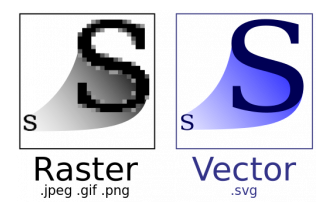
\includegraphics[width=0.4\textwidth]{rasterVsVektor.png}
    \caption{Vergleich Rastergrafik Vektorgrafik}
    \caption*{Quelle: \url{https://helpcenter.shirtigo.de/wiki/druckmotiv/vektorgrafik/\#:\~:text\=Grundlage\%20einer\%20Vektorgrafik\%20bilden\%20die,wie\%20Kurven\%2C\%20Kreise\%20oder\%20Polygone}}
\end{figure}

Illustrator wurde in \FF für die Erstellung von Icons, Symbole, Sticker und Plakate verwendet. Beispielseise ist es für Sticker besonders wichtig in einem vektorbasierten Programm zu arbeiten, da mit Photoshop ein Qualitätsverlust je nach Skalierung auftreten kann, was insbesondere für Druck ungeeignet ist. Mit Illustrator ist es möglich in einem CMYK-Farbmodus zu arbeiten, welcher für Druck üblicherweise verwendet wird, da Drucker mit einem CMYK-Farbprofil arbeiten, im Vergleich zu Bildschirmen im RGB-Farbprofil.

\section{Grafik und Design}

\begin{coolQuote}
    Design unterscheidet sich von Kunst in einem zentralen Punkt: es muss einen Zweck haben.
\end{coolQuote}
\zid{7prinzipe}

Mockups
helfen
, um
die
Funktionalität, Ästhetik und Benutzerfreundlichkeit eines Spiels zu visualisieren und zu testen. Es gibt viele Möglichkeiten, um ein Mockup zu erstellen, wie beispielsweise mit Papier und Bleistift, um einen groben Überblick zu erschaffen. Für große Applikationen werden allerdings Programme wie Adobe Xd oder Figma verwendet, da somit eine konsistente und dynamischere Arbeitsweise erzielt. Für \FF ist es wichtig, dass ein Programm verwendet wird, welches interaktive Seiten bauen lässt, die den Ablauf des Spiels simulieren.

\subsection{Navigation Bar}

Jedes moderne Videospiel hat ein Stück UI, welches immer sichtbar ist, um die wichtigsten Informationen, die für den Spieler relevant sind, anzuzeigen. Diese Grafik soll nicht zu viel Aufmerksamkeit zu sich ziehen, jedoch immer schnell sichtbar sein.
In \FF existiert eine Navigation Bar, bestehend aus einer schwarzen länglichen Leiste und drei Buttons, die zu den wichtigsten Menüs im Spiel führen, dem Hauptmenü, dem Rucksack und den Einstellungen. Die mit Photoshop Pinseln selbst gezeichneten Icons, helfen dem Spieler dabei noch schneller zu erkennen, welche Aufgabe der jeweilige Button hat, und merkt sich diese dadurch besser. In der schwarzen Leiste befinden sich die wichtigsten Informationen die für \FF relevant sind: die Lebensanzeige, den Ort, in dem sich der Spieler aufhält und wie viel Geld der Spieler bereits gesammelt hat. Beide Elemente haben eine raue Oberfläche, welche mit Texturen von
\quoted{Texturelabs.com}
texturiert wurden. Die Website bietet kommerziell kostenfreie Grafiken und Texturen, die über bereits existierende Grafiken gelegt werden können. Zusätzlich hat die schwarze Leiste als auch die Buttons eine raue Silhouette, um den Effekt zu verstärken.

\begin{figure}[H]
    \centering
    
\includegraphics[width=1.0\textwidth]{navigationsleiste.png}
    \caption{Navigationsleiste Grafik in \FF}
\end{figure}

Die Navigation Bar ist immer sichtbar, außer – wenn der Spieler verloren hat – im Death-Screen und während eines Kampfes. Während einem Kampf ist eine leicht abgeänderte, kleinere Variante der Navigation Bar zu sehen, da beispielsweise die Option
\quoted{zum Titel zurückzukehren}
nicht mehr verfügbar ist. Allerdings werden weiterhin die Lebenspunkte, das Deck und das bereits gesammelte Geld, angezeigt.
Sogenannte \quoted{Hover-} und \quoted{Active-States} geben dem Spieler ein Feedback, wenn sie mit der Navigationsleiste interagieren. Beispielsweise wird der Backpack-Button heller, sobald man mit dem Mauszeiger auf ihn fährt, um den Spieler mitzuteilen, dass dieser klickbar ist und eine Aktion auslöst. Sobald der User auf den Knopf drückt, erscheint einerseits das Rucksack UI, aber auch wird der Backpack-Button hinausgezogen. Das visualisiert, dass der Rucksack gerade offen ist, beziehungsweise dieser Knopf ausgewählt wurde.

\subsection{Map Mockup}

Angefangen mit einem simplen Wireframe, bestand das Mockup vorerst aus Events – das sind kleine Punkte auf der Karte – welche mit Strichen verbunden wurden, die einen Weg durch verschiedene Landschaften bilden. Es wurde mit Placeholder Texturen gearbeitet, um ein grobes Bild des Gameplays zu erstellen. Das UI hatte zuerst einige Elemente mehr, wie beispielweise eine Legende, die beinhält, die alle Events auf der Karte erklärt oder eine Minimap, die einen Überblick über die ganze Karte zeigt. Die Elemente wurden im Laufe der Zeit weggelassen, da diese Grafiken immer sichtbar wären und dadurch das UI an Informationen überfluten, die nicht immer benötigt werden würden.

\begin{figure}[H]
    \centering
    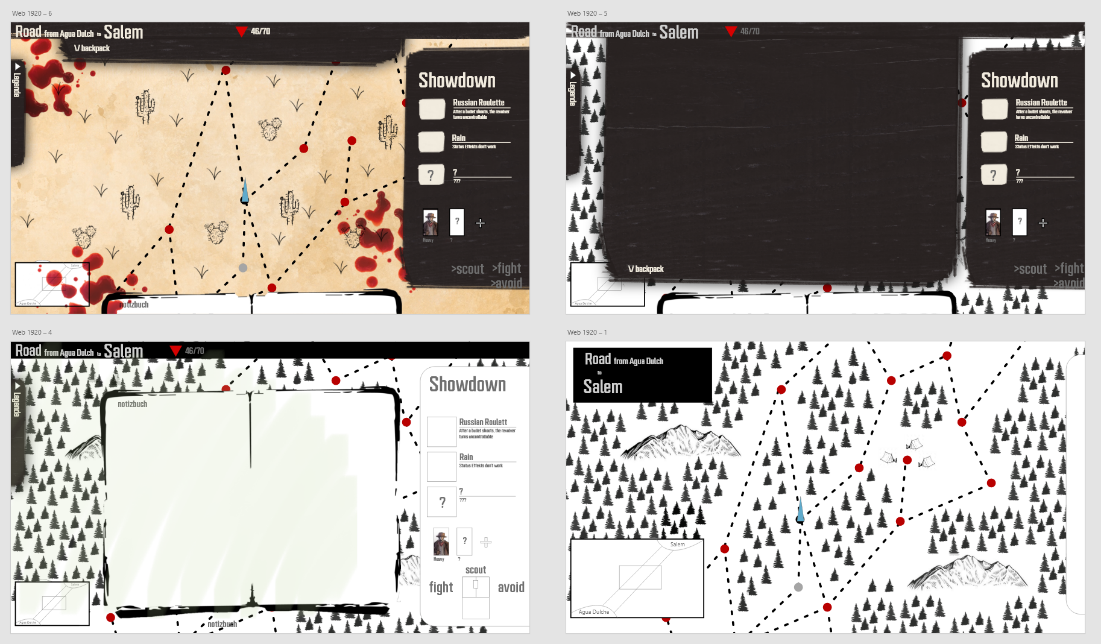
\includegraphics[width=0.8\textwidth]{altesMockup.png}
    \caption{Alte Version des Map Mockups}
\end{figure}

Es wurden über die Zeit viele Versionen von Texturen erstellt, da wir erst im Laufe der Diplomarbeit den passenden Stil entwickelt und gefunden haben. Beispielsweise ist in der aktuellen Version des \FF Mockups eine Textur für den Boden gezeichnet worden, die einen nahtlosen Übergang hat, damit diese unendlich oft aneinandergelegt werden kann. Da sich \FF einerseits in einer Wüstenlandschaft abspielt, mussten Kakteen, Skelette oder Häuser gezeichnet werden, da sie in einer Wüste üblich sind.

\begin{figure}[H]
    \centering
    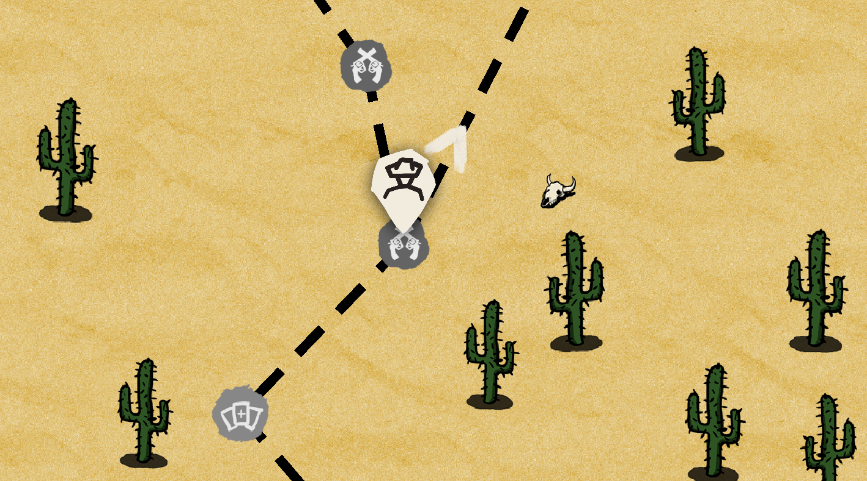
\includegraphics[width=0.8\textwidth]{mapAusschnitt.png}
    \caption{Ausschnitt der aktuellen Map}
\end{figure}

Das Event Popup ist das wichtigste Element, welches auf der Map sichtbar ist. Das Popup ist jedes Mal sichtbar, wenn der Spieler sich auf ein Event bewegt. Nehmen wir als Beispiel einen Kampf: Sobald der Spieler sich auf eines der kleinen Roten Symbole bewegt, welche mit einem Revolver Icon gekennzeichnet sind, erscheint auf der rechten Seite des Bildschirms das Showdown Fenster, welches dem Spieler die Informationen anzeigt, die für den Kampf relevant sind. Die folgenden Bilder zeigen die Entwicklung des Zeichenstils des User Interfaces.

\begin{figure}[H]
    \centering
    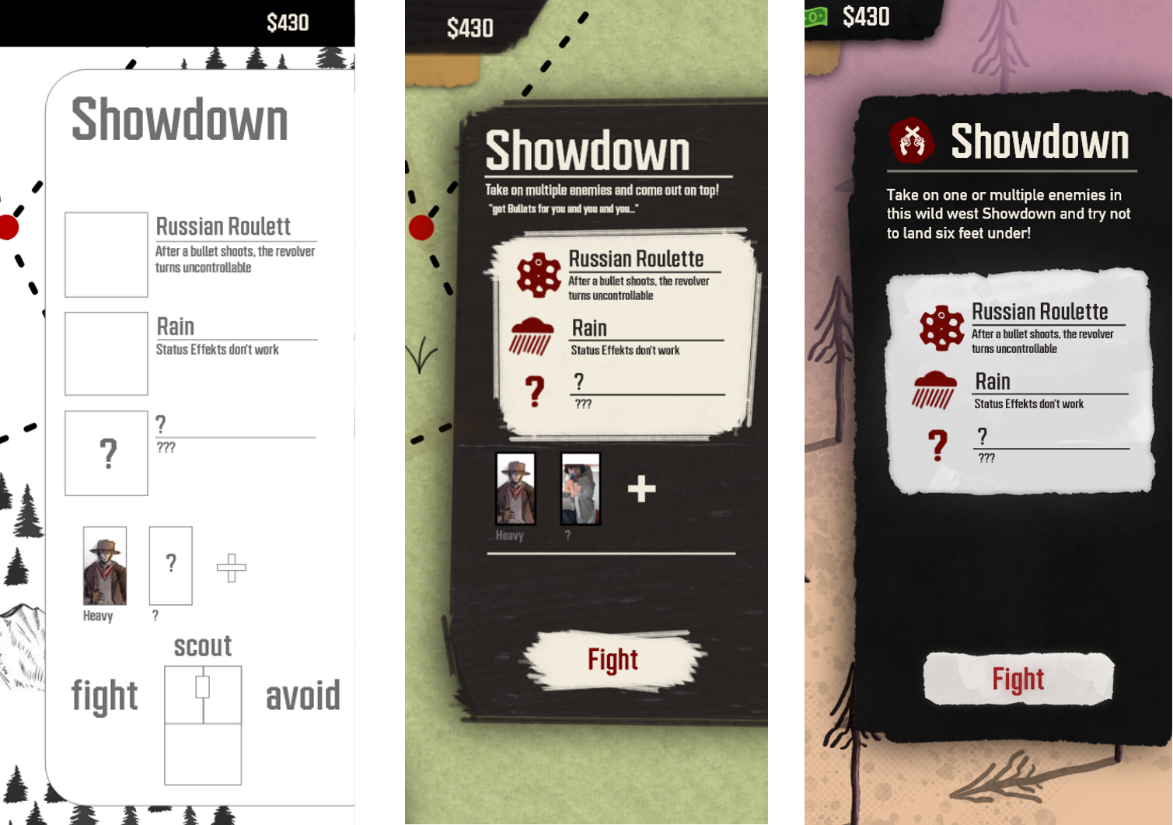
\includegraphics[width=1.0\textwidth]{showdown.png}
    \caption{Entwicklung des Showdown Fensters}
\end{figure}

Die Gestaltungsprinzipien sind in jeder Grafik in \FF wiederzufinden. In dem Popup ist erkennbar, dass die
Information in der weißen Box zusammengehört, aufgrund des Gesetzes der Nähe. Mit der Trennlinie wird weiters betont
, dass das Revolver Icon und das Wort Showdown der Titel für dieses Event sind. Auch das Gesetz der Ähnlichkeit zeigt
sich in der schwarzen Fläche, der weißen Box, als auch dem Button, da diese alle denselben rauen Zeichenstil haben.
Der Fight-Button hat sich mit der Zeit der Entwicklung vergrößert, da ein Button, der oft von dem Spieler betätigt
wird, schnell und einfach zugängig sein sollte. Ebenfalls wurde ein Hover State erstellt, damit der Spieler schnelles
Feedback zu seinen Aktionen erhält. Der einfachste weg einen Hover Zustand zu erstellen ist, indem die Farben einfach
getauscht werden, da diese weiterhin dem Farbschema treu bleiben und sich stark genug von dem originalen Knopf ohne
Hover Status abheben. \zit{btnHoverStates}

\begin{figure}[H]
    \centering
    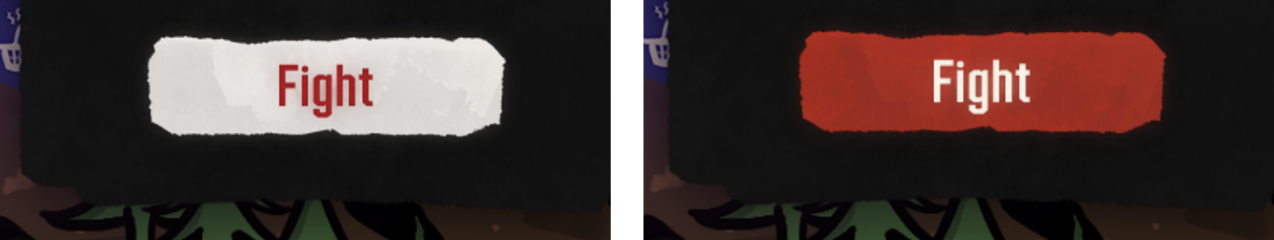
\includegraphics[width=1.0\textwidth]{fightButton.png}
    \caption{Hover Zustand des Fight Buttons}
\end{figure}

\subsection{Encounter Mockup}

Das Layout der Buttons und des Revolvers spielen eine wichtige Rolle in \FF. Das Encounter Mockup, auch Kampf, Showdown oder Fight UI genannt, wurde wie das Event Popup im Laufe der Diplomarbeit mehrmals von Grund auf neu gebaut, aufgrund Stil- und Game-Design Änderungen. Insgesamt wurde drei Mal das Encounter UI neugestaltet. Nach vielem Experimentieren kam es zur Conclusio, dass der Revolver – das Spielfeld – in der Mitte des Bildschirms sein muss, da dieser am meisten verwendet wird.

\begin{figure}[H]
    \centering
    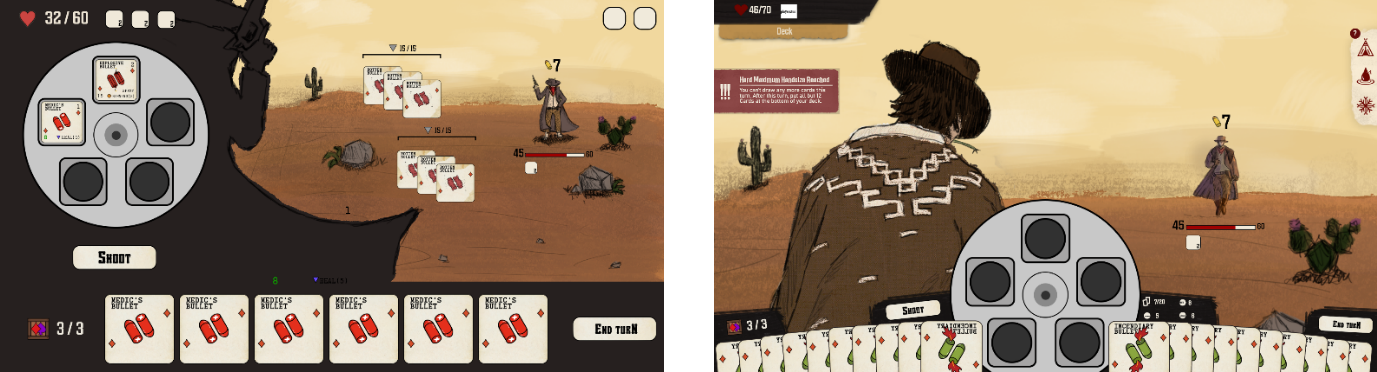
\includegraphics[width=1.0\textwidth]{altVsNeuEncounter.png}
    \caption{Altes versus verbessertes Encounter Mockup}
\end{figure}

Die Karten spielen eine genauso große Rolle. Für Kartenspiele – ob in Realität oder in Videospielen - ist es üblich, dass die Karten in einer Hand sind. Aus diesem Grund ist es die optimale Wahl, die Karten links und rechts von dem Revolver zu platzieren. Indem die Karten näher aneinander sind und sich überlappen, wirkt es mehr wie eine Hand, die die Karten hält. Damit sich die Karten auch gut voneinander abheben und genug Kontrast entsteht, wird ihnen ein Schlagschatten zugewiesen.

\begin{figure}[H]
    \centering
    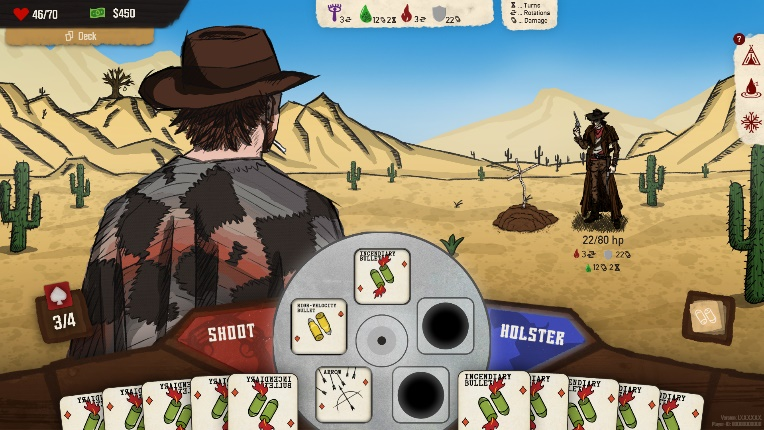
\includegraphics[width=0.6\textwidth]{finalerEncounter.jpeg}
    \caption{Finale Version des Encounter Mockups}
\end{figure}

Die alten Versionen des Encounter Mockups weisen wenige Texturen auf, weshalb dadurch nicht dem rustikalen western Stil von \FF entsprechen. Es wurde sich dafür entschieden, dass die Reserves- und Deck-Inseln getrennt von der Holzleiste im unteren Bereich des Bildschirms sind, da ansonsten die Holzleiste zu viel Fläche des Bildschirms einnehmen würde und das Hovern von Karten manchmal die Reserves verdecken würden. Mit einer Animation, die die Inseln schweben lässt, bringen diese zusätzliche Dynamik für das Auge.

Die Shoot und Holster Buttons, oder auch End Turn Button genannt, waren in den vergangenen Versionen des Mockups ungleichmäßig platziert. Da beide Aktionen eine wichtige Rolle spielen, wurde sich dafür entschieden, dass die neu entworfenen Buttons seitlich aus dem Revolver stehen sollten, sodass sie einfach zugängig und groß genug seien können.
Das \quoted{Parry} Mockup ist Teil des Encounter Mockups. Wenn ein Gegner am Anfang seines Spielzuges dem Spieler schaden zufügen möchte, hat die Spieler die Option den Angriff zu blockieren. Um diese Aktion für den Spieler zu intuitiv wie möglich zu gestalten, tauschen sich die vorherigen Buttons, die aus dem Revolver standen, mit einer Animation. Um die Spieler weiter aufmerksam auf diese Situation zu machen, wird mit einem Ton und Vignetten der Effekt verstärkt. Das baut Spannung auf und teilt dem Spielenden mit, dass dieser gerade vor einer wichtigen Entscheidung steht. Zusätzlich befindet sich in der Mitte des Bildschirms ein Erklärungstext zu der Aktion.

\begin{figure}[H]
    \centering
    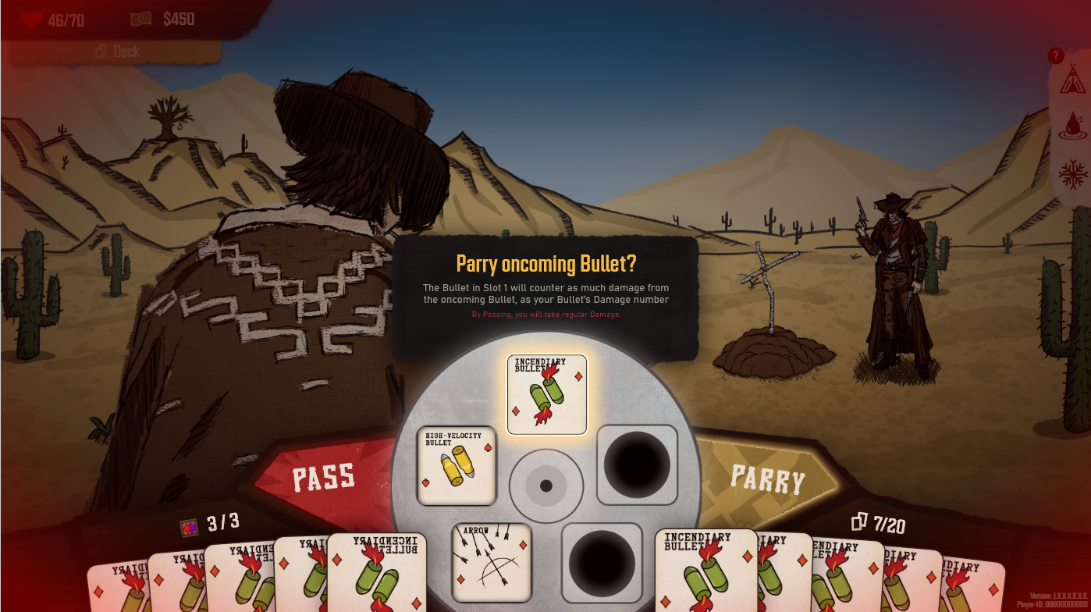
\includegraphics[width=0.8\textwidth]{parryMockup.png}
    \caption{Parry Mockup}
\end{figure}

Auch das Gesetz der Ähnlichkeit wurde beim Entwerfen des Mockups angewandt. In der linken oberen Ecke wird die Lebensanzeige und das Geld auf demselben schwarzen Balken angezeigt, der in jeder anderen Szene im Spiel zu sehen ist, um Spielern mitzuteilen, dass es hierbei um dieselbe Lebensanzeige handelt, welche für den Kampf und das strategische Handeln wichtig ist. Durch das Gesetz der Ähnlichkeit zeigt sich, dass die kürzere Leiste im Kampf dieselbe ist, wie die große Leiste auf der Map.

\begin{figure}[H]
    \centering
    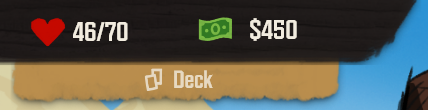
\includegraphics[width=0.8\textwidth]{navigationbarEncounter.png}
    \caption{Status Bar in kurzer Variante während des Kampfes}
\end{figure}

Statuseffekte werden durch Karten oder Gegner-Angriffe dem Spieler hinzugefügt. Beispielsweise zeigt folgendes Bild die Statuseffekte Bewitched, Poison, Burning und die Anzahl an Schild am oberen Rand des Bildschirms während dem Kampf. Es wurde sich dafür entschieden eine helle Hintergrundfläche im Stil eines Papiers hier zu verwenden, da ein dunkler Hintergrund die Komposition einengen und einen Rahmen setzen würde, was in diesem Fall unpassend wäre, da der Hintergrund der Elemente verhältnismäßig hell ist. Rechts im Bild zu sehen sind die
\quoted{Encounter Modifier}.
Das Sind Effekte, die den gesamten Kampf beeinflussen können. Diese werden auf derselben Papiertextur dargestellt, allerdings zeigt sich die Beschreibung der einzelnen Encounter Modifier erst, wenn der Spieler mit dem Mauszeiger über die Grafik fährt. Im Normalzustand sind nur die Icons zu sehen, um so wenig Platz wie möglich aufzubrauchen, da sonst das User Interface zu überladen und eventuell sogar überfordernd wirkt für die Spielenden.

\begin{figure}[H]
    \centering
    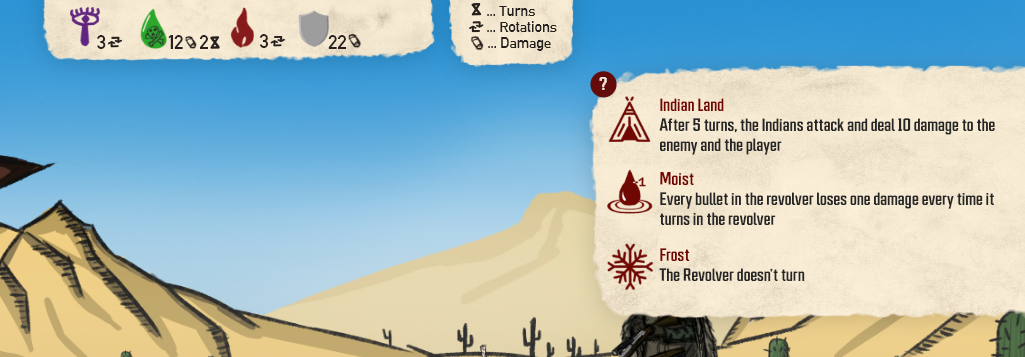
\includegraphics[width=0.9\textwidth]{statusEffekte.png}
    \caption{Statuseffekte und Encounter Modifier}
\end{figure}

\subsection{Backpack Mockup}

Das Backpack beinhält die Karten, die der Spieler über die Zeit gesammelt hat. Es wird mittels dem Backpack Button ge
öffnet, welcher mit einer Ease In und Ease Out Animation in das Bild gezogen wird. Wenn eine Animation erhebliche
Bildschirmänderungen mit sich bringt, beispielsweise wenn ein modales Fenster angezeigt wird, kann eine Dauer von 200
–300 ms angemessen sein. Je weiter sich ein Element bewegen muss, desto wichtiger ist es, dass dies reibungslos und
ohne Erschütterungen geschieht (besonders für bewegungsempfindliche Menschen, wie z. B. Benutzer mit Epilepsie oder
Gleichgewichtsstörungen) \zit{designPrinzipien}. Aus diesem Grund ist es wichtig, dass Animationen in \FF
minimalistisch gehalten werden.

Eine simple Box um mehrere Objekte, zeigt unserem Gehirn, dass die Information darin zusammengehört. Genau dasselbe
wird beim Backpack UI in \FF angewendet. Mit dem braunen, lederartigen, Rucksack-ähnlichem Asset wird das Gesetz der
Geschlossen übermittelt. Dieses Konzept möge hier angewendet werden, da unser Gehirn in der Wahrnehmung Formen erg
änzt, sodass geschlossene Figuren entstehen \zit{gestaltGesetze}. Der Name der Decks ist änderbar. Aus Usability
technischen Gründen
befindet sich der Knopf zur Bearbeitung direkt neben dem Namen, um es für den Spieler zu schnell zugänglich zu machen wie möglich, genauso wie alle anderen wichtigen Funktionen des Backpacks, wie die Sortierfunktion und die Wechselfunktion zwischen den verschiedenen Decks.

\begin{figure}[H]
    \centering
    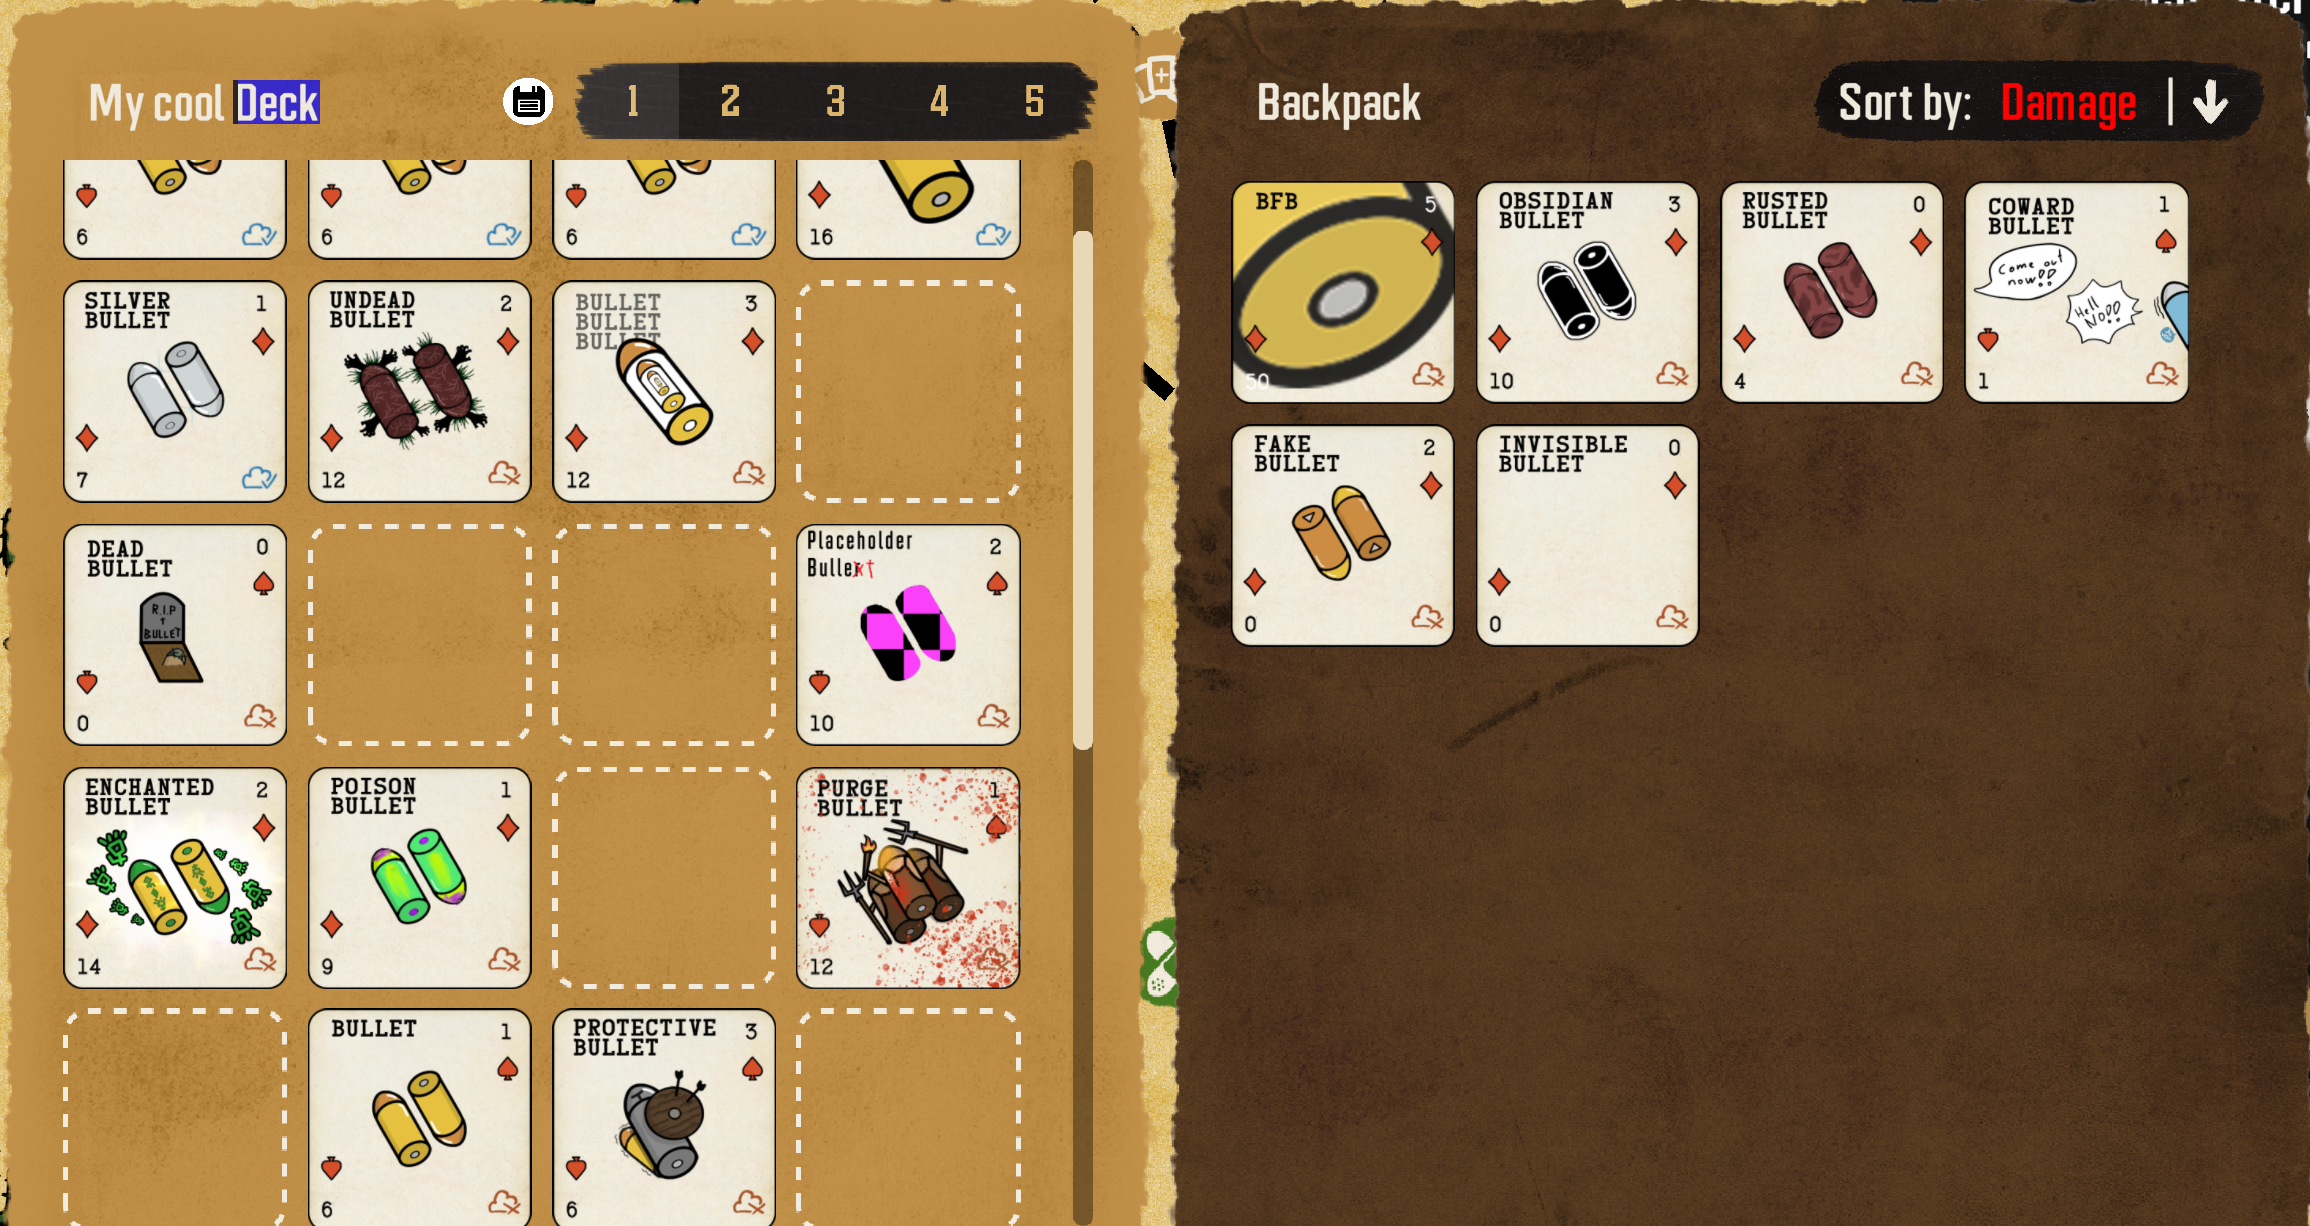
\includegraphics[width=1.0\textwidth]{backpack.png}
    \caption{Screenshot des Backpack UIs}
\end{figure}

\subsection{Dialog Mockup}

Bei vielen Videospielen ist es üblich, dass sich auf dem Dialog Screen einerseits ein Textfeld und die Person mit der interagiert wird, befinden, wie beispielsweise auf
\quoted{Game UI Database} – eine Website die User Interface Screenshots von Videospielen zur Schau stellt – zu erkennen ist. Für die User Experience ist zu beachten, dass die Texte von den NPCs nicht zu lang sein dürfen, was auf einigen Screenshots der Website zu erkennen ist. Ein bis Zwei Zeilen sollten maximal pro Klick angezeigt werden. Dadurch wird die Gefahr verringert, dass Spieler den Text überfliegen. Weiters ist das Namenschild des NPCs ist auf derselben Seite wie der NPCs. Dadurch wird besser übermittelt, dass beispielsweise im folgenden Screenshot die Hexe den Namen
\quoted{Evil Witch} im Spiel trägt.

\begin{figure}[H]
    \centering
    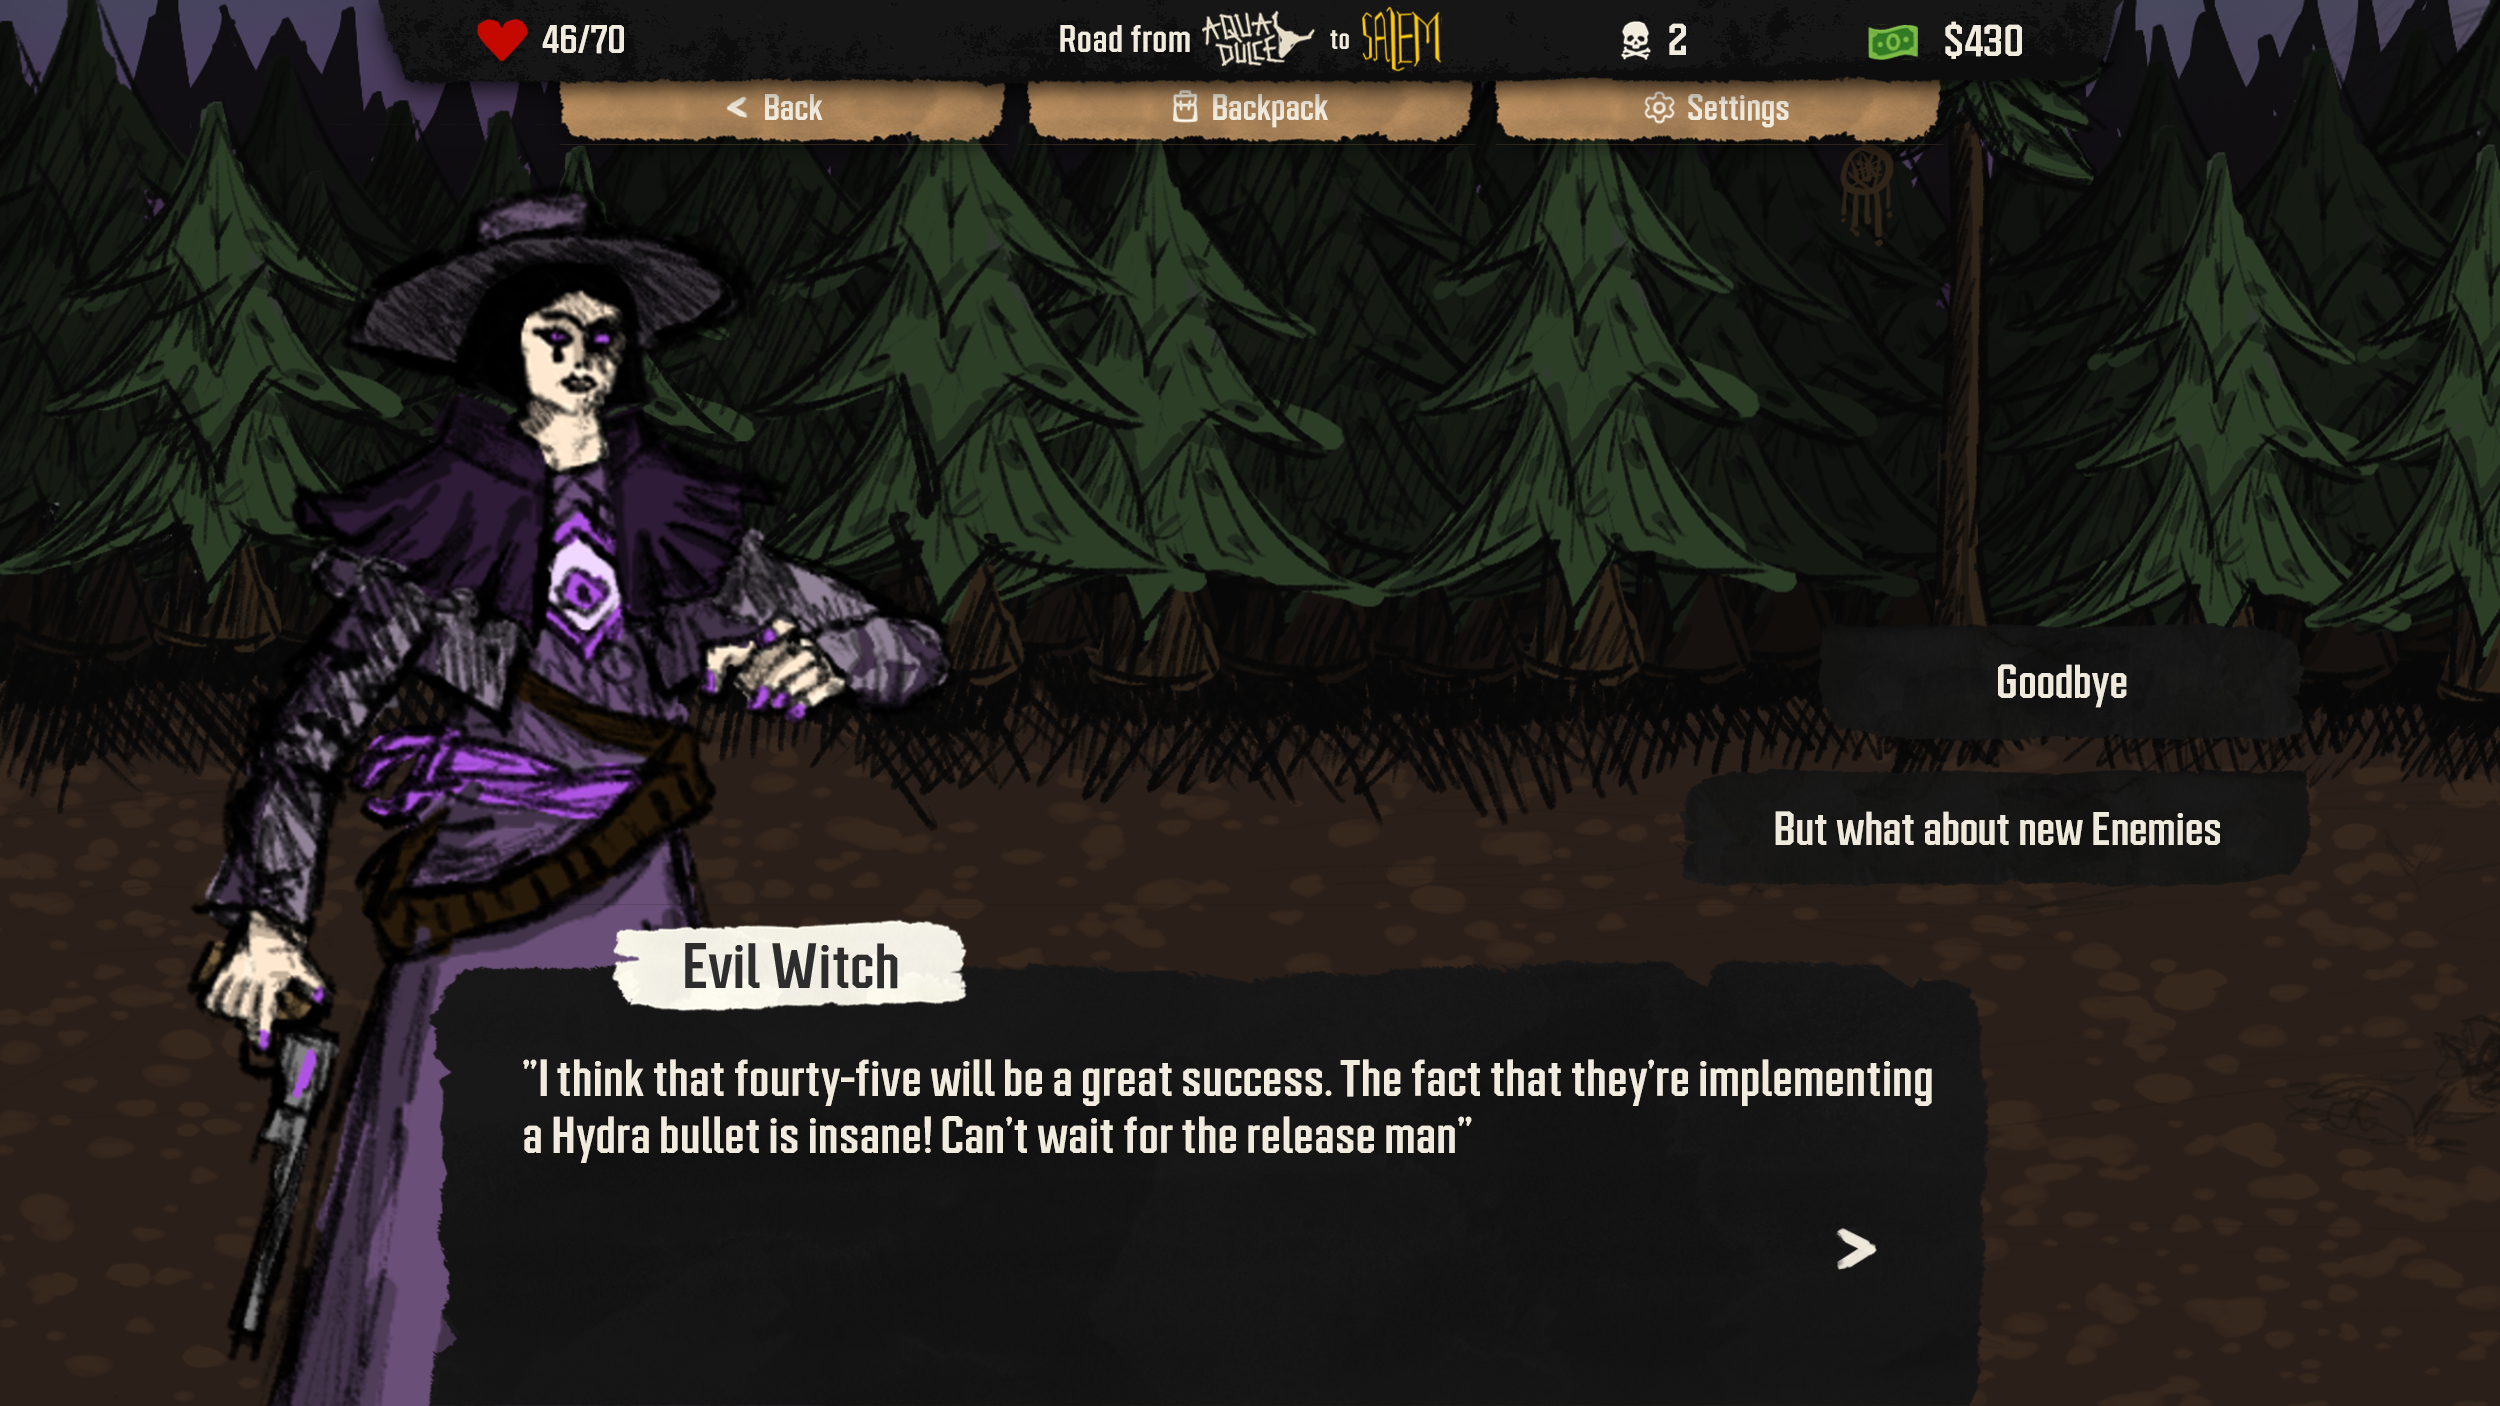
\includegraphics[width=1.0\textwidth]{witchInteraktion.png}
    \caption{Interaktion mit dem NPC "Evil Witch"}
\end{figure}

\subsection{Title Screen und Death Screen}

Ein Videospiel ohne Titelbildschirm ist wie ein Buch ohne Cover. Der Erste Eindruck eines Spiels ist der wichtigste. Mit dem Title Screen kann eine gewisse Professionalität übermittelt werden und dem Marketing dienen, wenn dieser gut gelingt. Dieser wird sehr simpel gehalten und zeigt keine Besonderheiten, außer den Namen des Spiels und einem Text wie etwa
\quoted{Press to Start}.
Jedoch gibt es noch eine andere Art von Title Screen, nämlich das Menü-Basierte, wobei der Spieler unmittelbar nach dem Starten mehrere Optionen zur Auswahl hat, wie
\quoted{Credits} oder \quoted{Settings}.  Der Title Screen von \FF besteht
aus dem \FF Logo und den Optionen Continue, Abandon Run, Reset Game, View Credits und Quit. Die Reihenfolge dieser Buttons ist ein großer Bestandteil der User Experience. In anderen Videospielen ist sichtbar, dass die erste Option dafür da ist, um das Spiel zu starten, beziehungsweise um in \FF auf die Map zu kommen, während die letzte Option in der Auflistung dazu dient, das Spiel zu schließen, da ein Spielentwickler möchte, dass der User das Spiel so lange wie möglich beschäftigt ist und nicht auf die Idee kommt das Spiel zu schließen.

\begin{figure}[H]
    \centering
    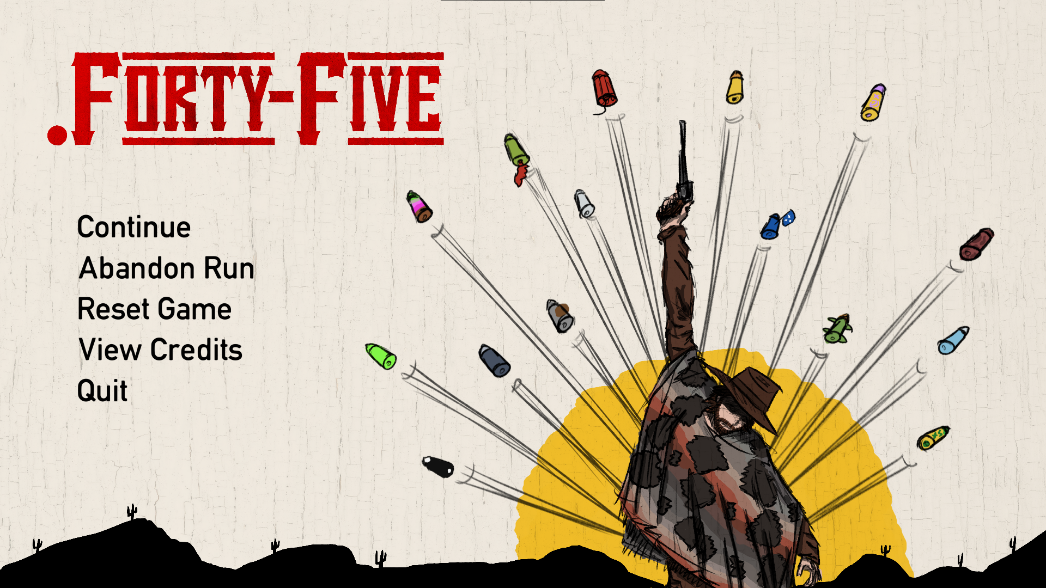
\includegraphics[width=1.0\textwidth]{titlescreen.png}
    \caption{Title Screen von \FF}
\end{figure}

Der Hintergrund für den Title Screen wurde in Adobe Photoshop erstellt, und die Grafiken digital per Hand gezeichnet
. Die Idee war es, ein Mural nachzustellen, angepasst auf \FF. Ein Mural ist eine Art der Wandmalerei, bei der das
Bild auf Wänden oder Decken gemalt wird. \zit{wandmalerei} Die Textur, die über das gesamte Artwork gelegt wurde,
unterstützt diesen
Effekt im Title Screen. Das Spiel dreht sich rund um die Bullets. Daher ist es wichtig, dass die Bullets gut im Title Screen vertreten sind und präsentiert werden. Der Titelbildschirm steht auch als Gegenstück zu dem Death Screen. In dem Start Screen wird ein Sonnenaufgang gezeigt, während andererseits ein Spieler im Death Screen – wenn dieser verloren hat – sich in einem Loch befindet, wie folgender Ausschnitt aus dem Spiel zeigt. Dadurch wird Anfang und Ende des Spiels besser präsentiert. Der Death Screen soll zeigen, wie der Spieler gerade begraben wird, nachdem ihm die Leben in einem Kampf ausgegangen sind. Da hauptsächlich nur Rot in diesem Bild vorkommt, wird dem Spielendem schnell übermittelt, dass es sich hierbei um eine Niederlage handelt, da die Farbe Rot oft mit dem Negativen verbunden wird. Es wurde kein auffälliger Button eingefügt, um aus dem Death Screen zu kommen, sondern nur ein kleiner Schriftzug, der dem Spieler hinweist, dass er mit einem Mausklick weiterkommt. Der Haupt Fokus soll auf dem großen Schriftzug
\quoted{A Terrible Fate} und die Zeichnung im Hintergrund liegen.

\begin{figure}[H]
    \centering
    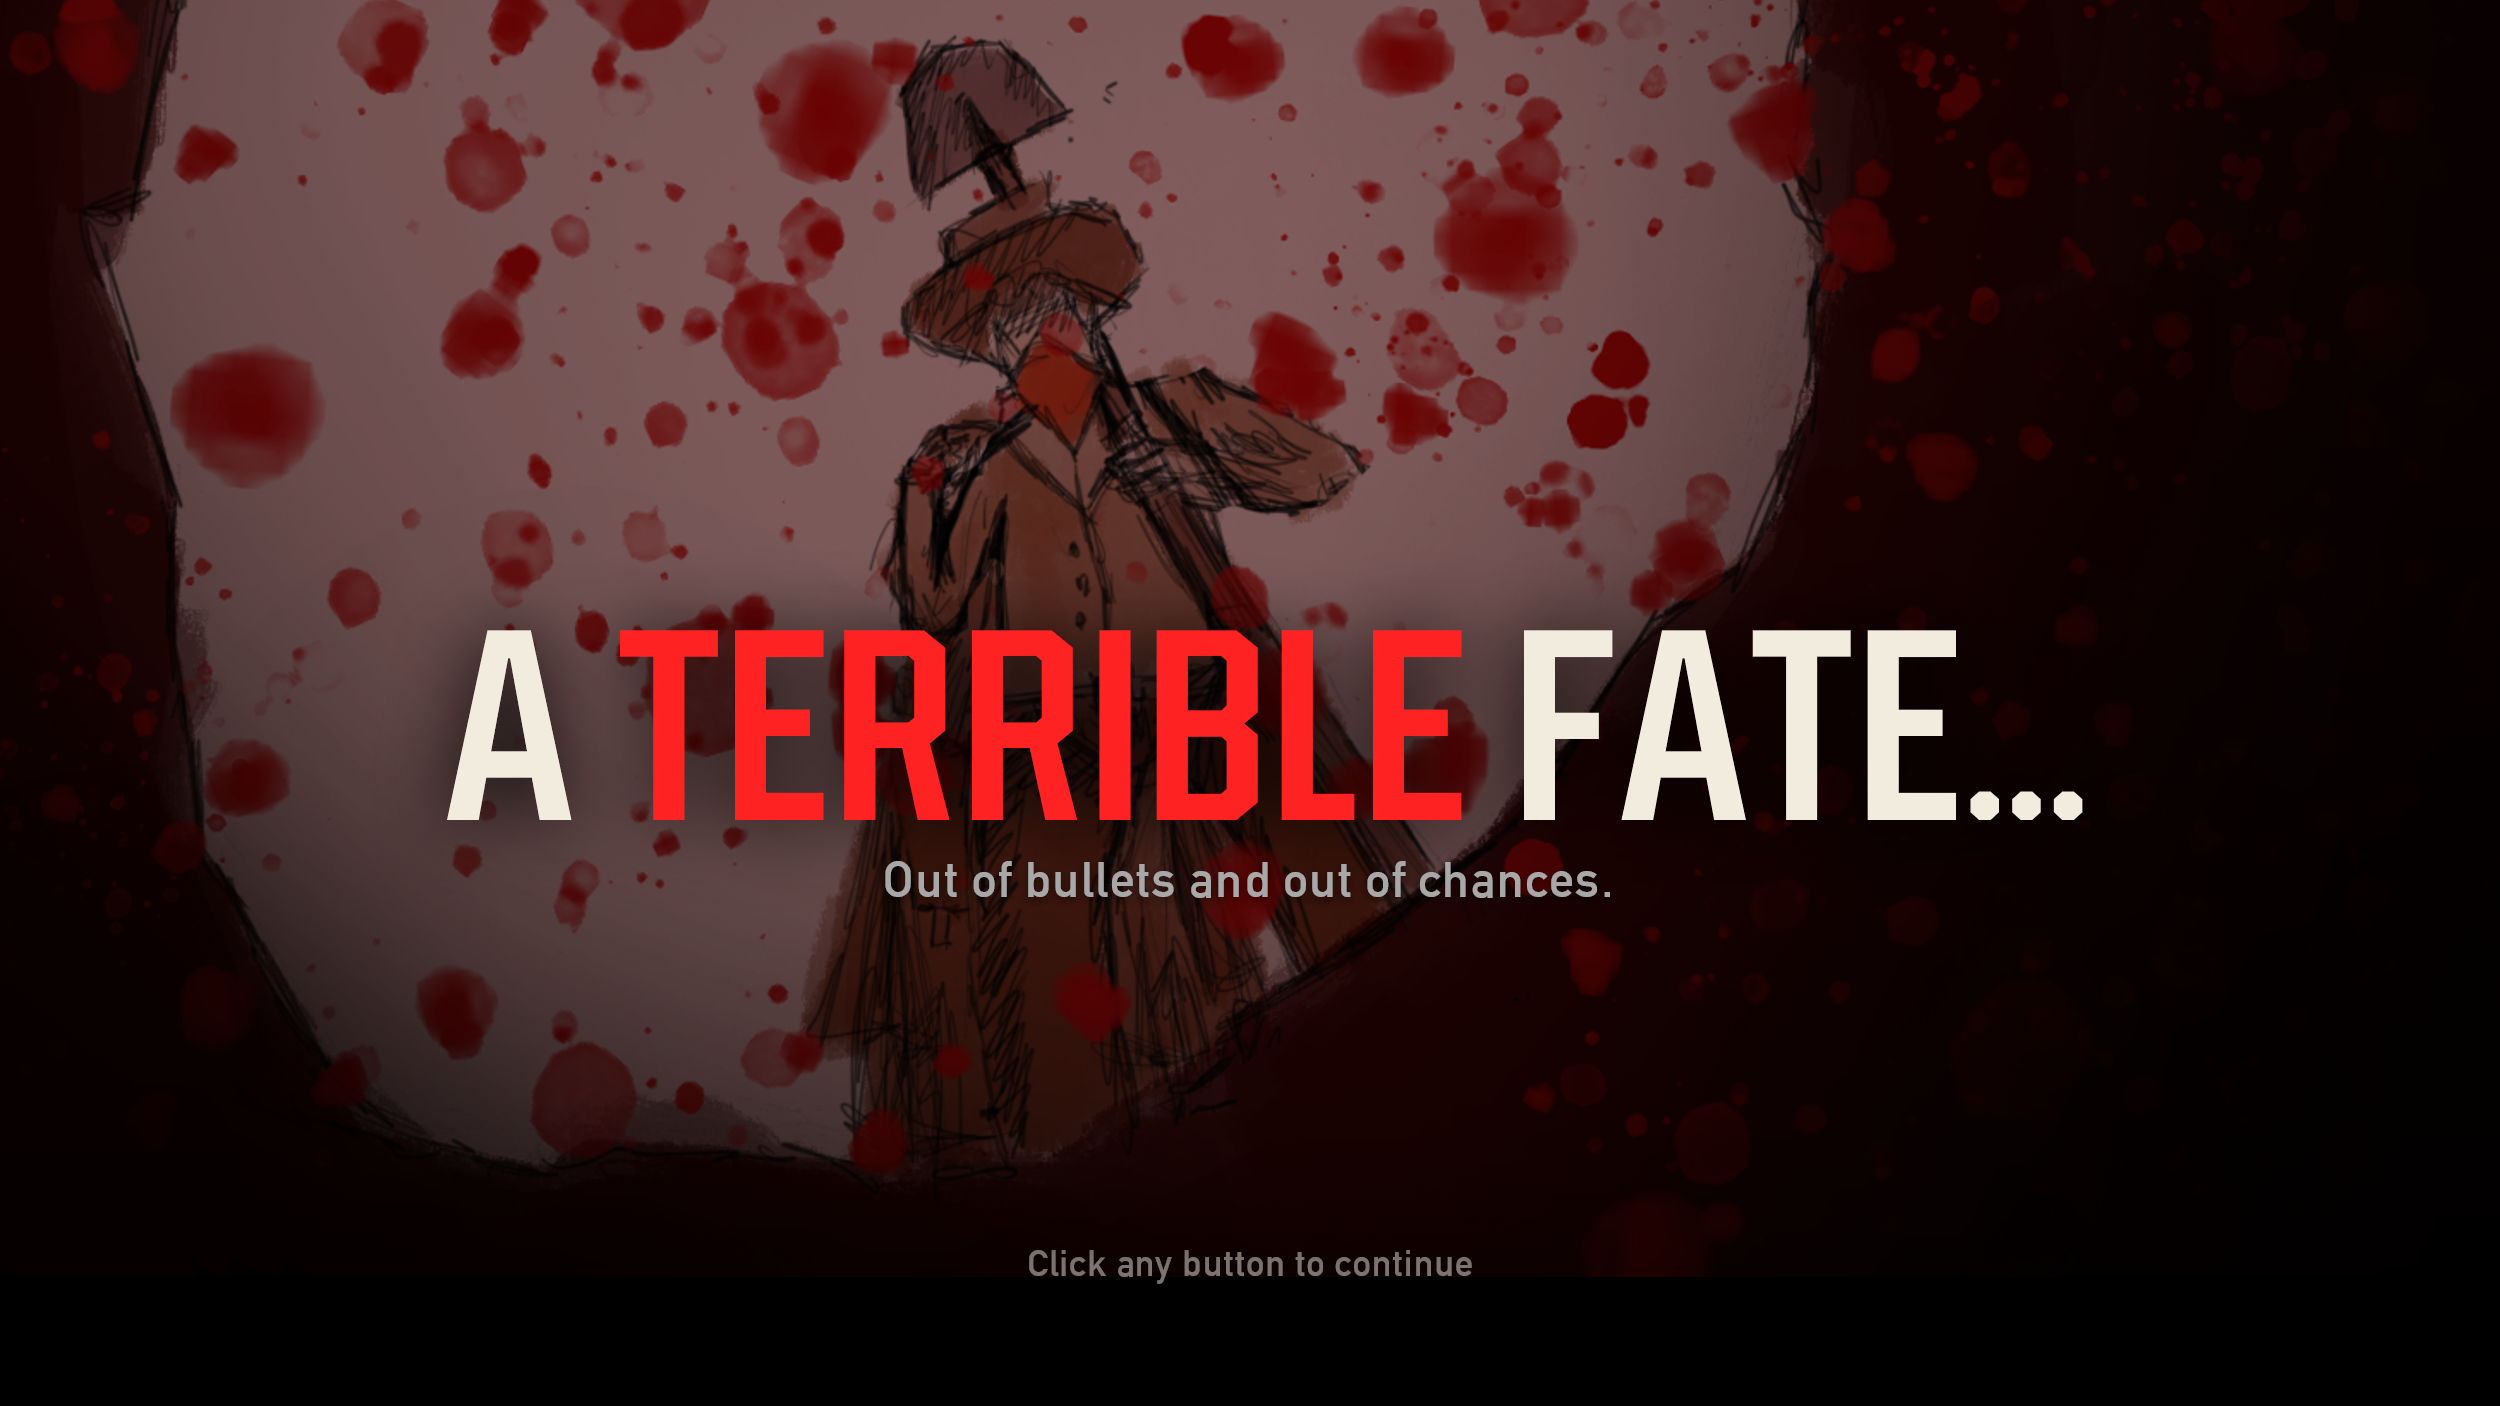
\includegraphics[width=1.0\textwidth]{deathscreen.png}
    \caption{Death Screen von \FF}
\end{figure}

\subsection{Map Event Mock-ups}

Auf der Map findet man verschiedene Events. Einen Shop, interagier bare NPCs und Orte, an denen sich der Spieler heilen oder eine neue Karte auswählen kann. Ähnlich zu dem Kampf, erscheint auf der rechten Seite des Screens ein Pop-up Fenster, indem man dieses Event starten, beziehungsweise den Ort betreten kann. Den einzelnen Ereignissen auf der Karte wurden Farben zugewiesen, damit der Spieler diese schneller erkennen kann. Die Icons der Events spielen eine große Rolle, da ein Spieler beim ersten Blick sofort erkennen muss, was er sich bei dem Ereignis ungefähr erwarten kann. Die Symbole wurden mit demselben Pinsel gezeichnet, wie die UI Elemente, um für Einheit im Design zu sorgen. Je simpler Icons sind, desto besser wird die Information übermittelt.

\begin{figure}[H]
    \centering
    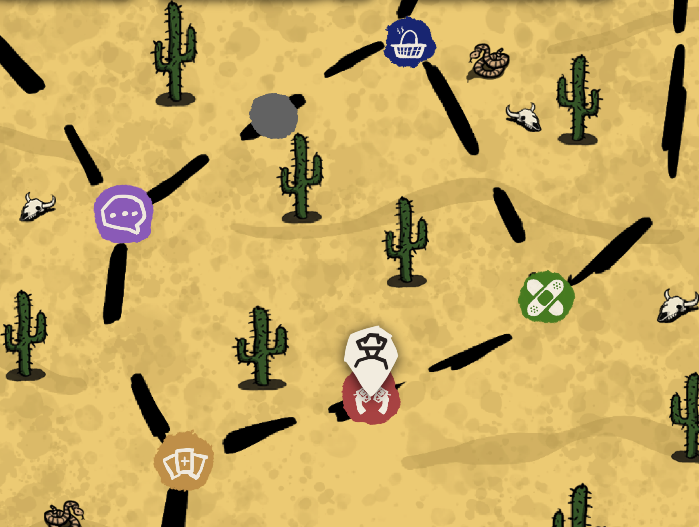
\includegraphics[width=1.0\textwidth]{ereignisseMap.png}
    \caption{Nahansicht der Ereignisse auf der Map}
\end{figure}

Der Shop zeigt auf der linken Seite den Händler, der einem die Ware verkauft, während sich auf der rechten Seite die Karten befinden, welche auf einer schwarzen Fläche hinterlegt sind. Um die Bullets von anderen Texten die Informationen zum Shop geben zu trennen, wird eine weiße Box hinter diese gelegt. Weiteres ist für die User Experience wichtig, dem Spieler mitzuteilen, dass dieser die Karten ziehen muss, um sie in den Rucksack oder das Deck zu legen. Daher befindet sich unten am Bild ein Informationstext, der die Funktionalität dem Spieler erklärt.

Bei einem weiteren Ereignis auf der Map, kann sich der Spieler eine von drei neuen Karten aussuchen, die er noch nicht besitzt. Das gleiche Event ist auch zusehen, nachdem der Spieler einen Kampf gewonnen hat. Damit der User weniger denken muss, wird hier dasselbe Prinzip verwendet wie beim Shop, als auch beim Rucksack, nämlich muss der Spieler seine ausgewählte Karte in sein Deck oder den Rucksack ziehen. Weiters besteht die Option auch keine Karte auszuwählen, wird dem Spieler allerdings nicht empfohlen, daher ist der Button für diese Entscheidung etwas versteckt und rot markiert, um zu signalisieren, dass dies vermutlich keine gute Entscheidung sei.

Sehr ähnlich aufgebaut ist das Heil Event. Im gleichen Stil aufgebaut ist ein Fenster zu sehen, nachdem man das Ereignis betreten hat, indem sich der Spieler zwischen zwei Heilungsoptionen entscheiden kann. Allerdings zieht hier der Spieler nichts in sein Deck oder in den Rucksack, sondern muss sich zwischen zwei Auswahlmöglichkeiten entscheiden. Daher ist es Usability freundlicher, einen Button zu haben, der die Auswahl bestätigt, den Spieler heilt und ihn wieder zurück zur Map bringt. Dem Spieler muss mitgeteilt werden, dass er bei diesem Event die zwei Heilungsoptionen anklicken kann, um eines davon auszuwählen. Daher ist ein
\quoted{Hover}- und \quoted{Active} Zustand vorhanden.

Das Letzte Event ist auch ein Heilevent, allerdings hat der Spieler hier keine mehreren Auswahlmöglichkeiten, sondern nur eine Option. Deswegen hat der Spieler hier keine Möglichkeit etwas auszuwählen, sondern nur einen Button, um sich zu heilen und zur Map zurückzukehren.

\begin{figure}[H]
    \centering
    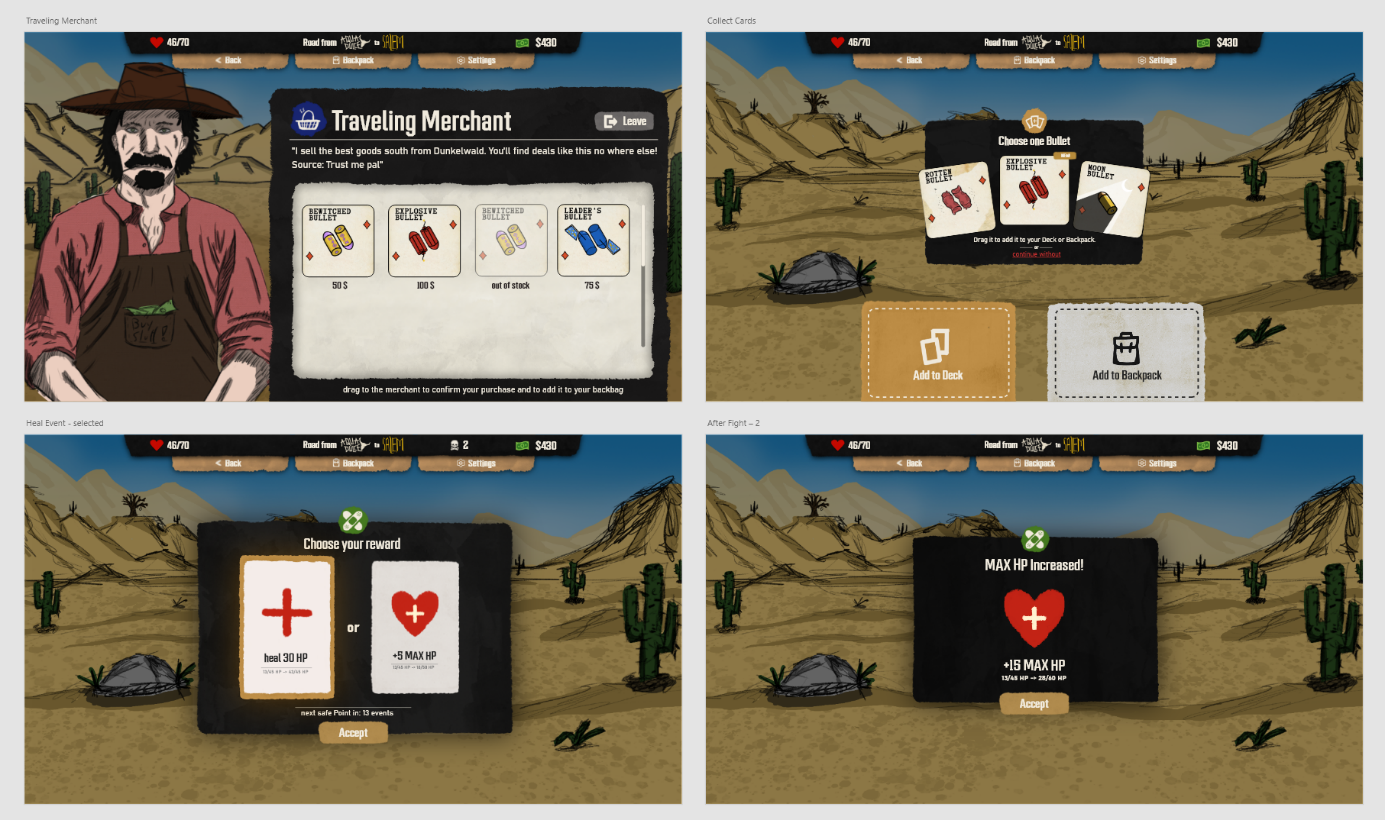
\includegraphics[width=1.0\textwidth]{mapEventsUI.png}
    \caption{Screenshot aus dem Mockup der Map Events}
\end{figure}

Für einen Wiedererkennungswert ist es wichtig für Einheit im Design zu sorgen. Die Hintergrundtexturen werden weiterverwendet und die Buttons sind wie im Screenshot zu sehen die gleichen. Weiters wird der Hintergrund von jedem Map Event abgedunkelt, damit der Fokus auf das Pop Up liegt, und nicht mit dem Hintergrund verschwimmt. Auch Erklärungstexte oder zusätzliche Informationen zu den Jeweiligen Events sind immer am Ende der Pop Ups zu finden. Alle diese kleinen Merkmale sorgen dafür, dass der Spieler nicht nachdenken muss und sofort erkennen kann, was passiert.

\subsection{Popups}

Der Begriff Popup stammt aus der Programmierung von Computersoftware. Ein \quoted{Pop-up} ist letztendlich ein Fenster oder eine grafische Benutzeroberfläche, die plötzlich auf dem Bildschirm erscheint. Diese Pop-ups können verschiedene Zwecke haben, wie beispielsweise Eingabeaufforderungen, Benachrichtigungen, Warnungen oder für sonstige Informationen. Meistens haben diese nur die Optionen
\quoted{Ja} und \quoted{Nein},
oder wenn das Pop-up nur eine Mittelung sei, nur einen
\quoted{Ok} Button \zit{dialogWiki}.

Auch in Videospielen ist dieser Begriff vertreten. In \FF gibt es Pop-ups im Tutorial des Spiels, bei sämtlichen Events auf der Map und nach Kämpfen. Beispielsweise ist im folgenden Screenshot das \quoted{Card Extraction Pop-up} zusehen. Dieses Pop-Up teilt dem Spieler mit, dass die in ein der vorherigen Road gesammelten Karten gespeichert wurden, da der Spieler es in die nächste Area geschafft hat, gespeichert wurden. Mit dem Symbol oben auf dem Pop-Up versteht der User schneller was für einen Screen er gerade sieht, und merkt sich für die Zukunft, dass dieser blaue Farbton für das Speichern der Karten in \FF verwendet wird.

Grundsätzlich ist jedes Pop-Up gleich aufgebaut. Ein schwarzer Texturierter Hintergrund, welcher mit Photoshop erstellt wurde, einem Titel, einem kurzen Erklärungstext auf der Unterseite, und einem Button, um das Fenster wieder zu schließen. Die Form der drei Flächen – schwarz, blau und weiß – wurden in Photoshop mit dem \quoted{Sketching Brush} Pinsel erstellt und danach mit dem
\quoted{Mad Ink} Pinsel in der Farbe Weiß texturiert. Dafür müssen die Pixel der Ebene in Photoshop fixiert werden, damit man nur innerhalb der Pixel der Ebene malt und nicht außerhalb. Danach stellt man den Pinsel auf 3\% Deckkraft und 70\% Fluss und fährt mit ihm einmal über die Fläche. Diese Methode bei der Erstellung von jedem Pop-Up angewendet. Der blauen Fläche wurde noch ein blau leuchtender Schlagschatten hinzugefügt, damit das Fenster etwas mehr an Tiefe bekommt und nicht mehr so flach und leblos wirkt.

\begin{figure}[H]
    \centering
    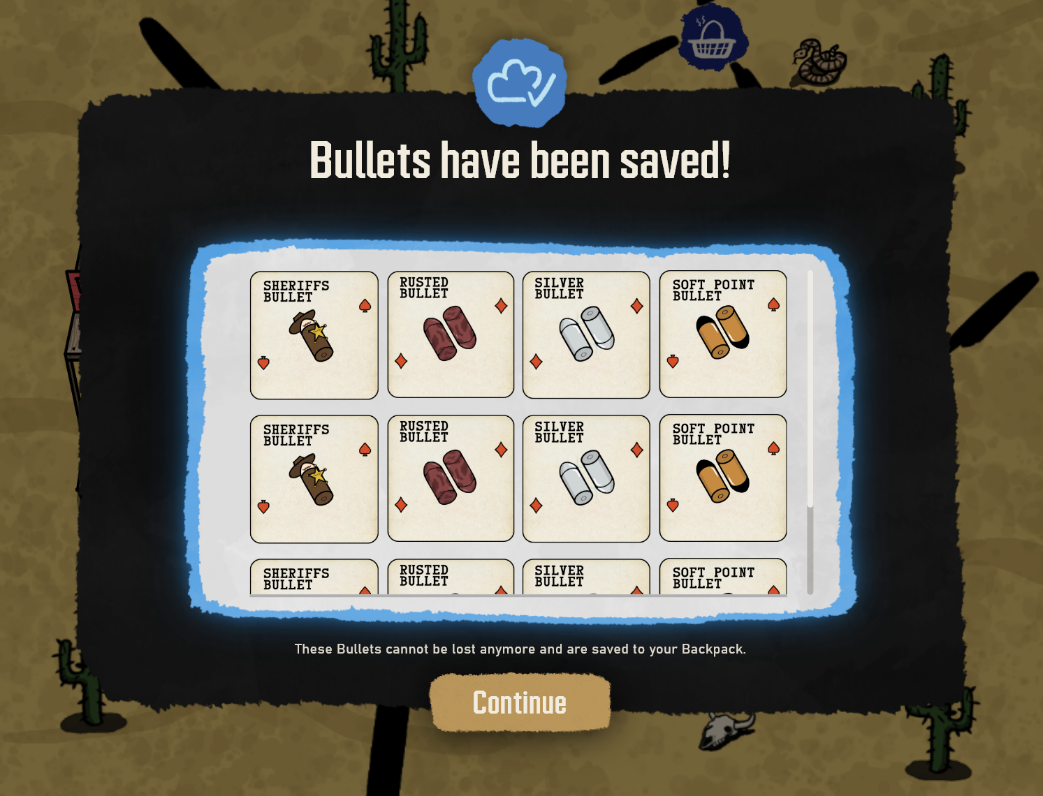
\includegraphics[width=0.5\textwidth]{cardExtraction.png}
    \caption{Card Extraction Pop Up}
\end{figure}

Eine weitere Art von Pop-Ups in \FF ist ein Fenster, in das der Spieler Karten ziehen muss, da dieser bereits zu viele Karten auf der Hand hat und welche ablegen, beziehungsweise zurück ins Deck legen muss. Da der Spieler vom Kampf es gewöhnt ist, die Karten in den Revolver zu ziehen, ist es hier am intuitivsten, den Spieler die Karten, die abzugeben sind, in eine Fläche zu ziehen. Dieser wird wie auf Folgendem Screenshot aus dem Mock-Up als Deckstapel angezeigt, damit der Spieler weiß, wohin die Karten gehen. Im Fall, dass der Spieler trotzdem nicht weiß was zu tun ist, stehen kurze Erklärungstexte auf dem Pop-Up. Letztendlich gibt es rechts unten einen Button, um die Auswahl an zurückgelegten Karten zu bestätigen, damit der Spieler nicht aus Versehen eine Karte abgibt, die er eigentlich noch behalten wollte.

\begin{figure}[H]
    \centering
    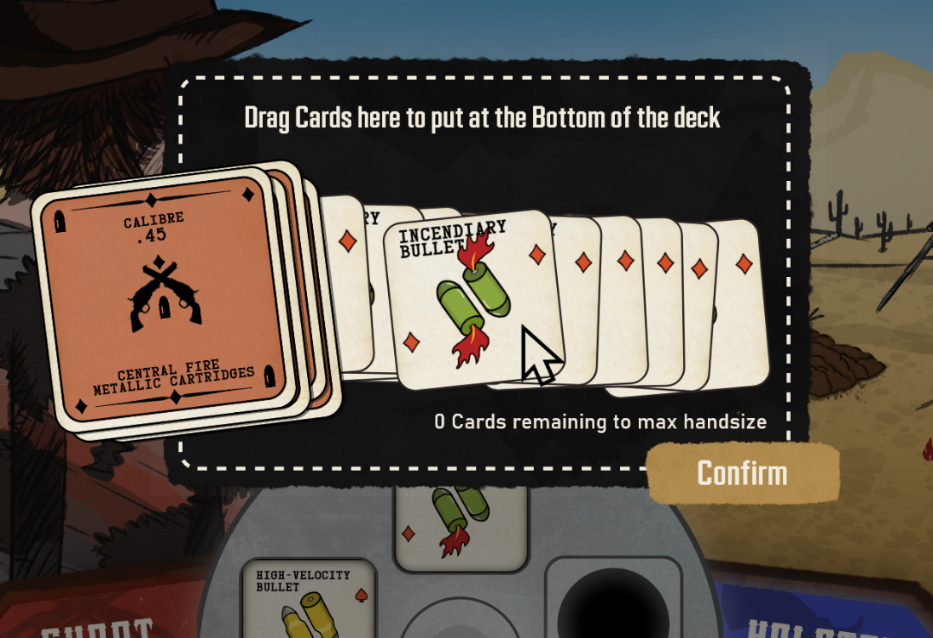
\includegraphics[width=0.5\textwidth]{encounterPopup.png}
    \caption{Pop-Up während des Kampfes}
\end{figure}

Ein Beispiel für ein Pop-Up, welches nur für Informationen dient, sind die sogenannten \quoted{Hover Details}. Für \FF ist es essenziell zu wissen, wie die Karten funktionieren und was ihre Effekte sind, daher müssen diese Informationen schnell zugänglich sein. Wenn der Spieler mit seinem Mauszeiger über eine Karte fährt, erscheint nach kurzer Zeit ein Pop-Up, welches nur aus Text besteht, welches die Karte beschreibt und dessen Effekte.

\begin{figure}[H]
    \centering
    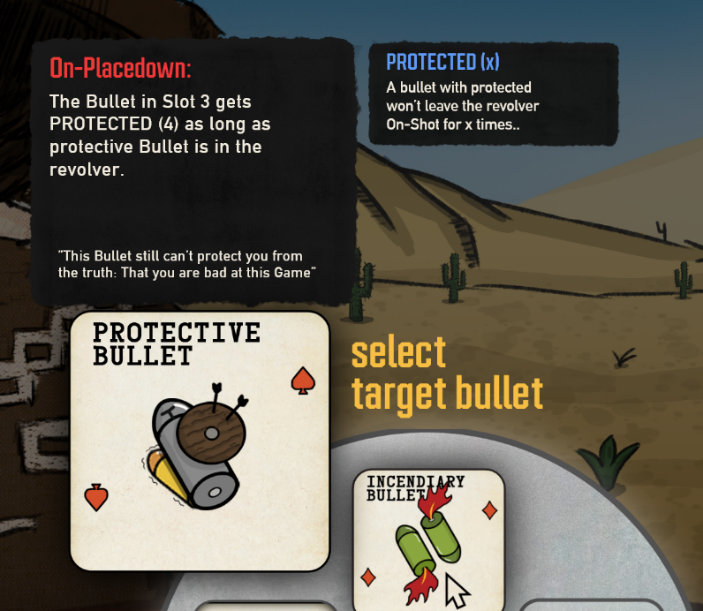
\includegraphics[width=0.6\textwidth]{hoverdetails.png}
    \caption{Beschreibung der Karte während Hover-Zustand}
\end{figure}

Während einem Kampf kommt es auch zu gegnerischen Angriffen, die besondere Auswirkungen auf den Kampf haben können, wie beispielsweise die Hexe, die die Revolver Drehrichtung des Spielers für die nächsten \quoted{x} Rotationen ändert. Damit der User das mitbekommt, erscheinen kleine Zeichnungen nacheinander, die im Comic Stil die Animation der Hexe zeigen. Dieses Pop-Up kommt zusätzlich zu den Grafiken mit einer Fläche, die die Aktion des Gegners erklärt und dessen Dauer anzeigt. Die Animation verschwindet nicht von selbst, sondern verschwindet erst nach einem Mausklick, um sicherzustellen, dass der Spielende die Information, die für den Kampf wichtig ist, mitnimmt.

\begin{figure}[H]
    \centering
    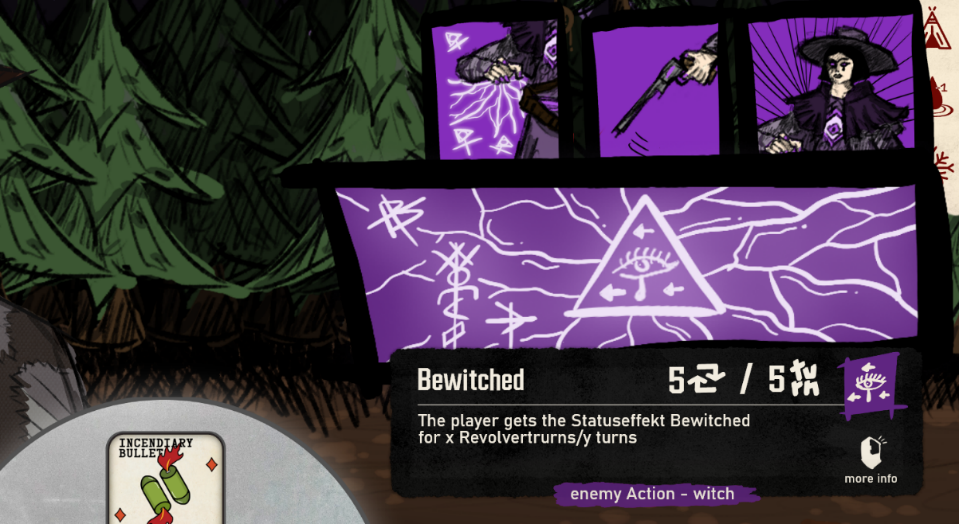
\includegraphics[width=1.0\textwidth]{enemyAction.png}
    \caption{Animation eines gegnerischen Angriffs}
\end{figure}

\subsection{Settings Menu}

Sobald ein Spieler ein Spiel gekauft hat, ist es wahrscheinlich, dass er seine ersten Erfahrungen in den
Einstellungen macht, bevor er überhaupt spielen wird. Für PC-Spieler ist die Überprüfung der Einstellungen, um
sicherzustellen, dass das Spiel ordnungsgemäß läuft, wahrscheinlich der erste Schritt, bevor das neue Spiel gestartet
wird. Ebenso können Streamer und YouTuber das Spiel im Voraus vorbereiten, einschließlich Lautstärke, um
sicherzustellen, dass ihr Publikum den besten ersten Eindruck von dem Spiel bekommt \zit{betterGameSettings}. Während
der Entwicklung
von \FF war es noch unklar, wie groß das Spiel letztendlich wird. Davon ist auch die Größe der Einstellungen abhängig. Daher wurde ein Einstellungen Menu mit Ankerpunkten vorausgeplant, falls die Einstellungen doch größer werden sollten. Das System von Ankerpunkten in den Einstellungen ist in vielen Spielen vertreten und hilft dem Spieler, schneller durch die Optionen zu navigieren. Beispielsweise verwendet das Videospiel \quoted{Armored Core IV: Fires of Rubicon} das selbe Layout wie das Einstellungen Menu von \FF.

\begin{figure}[H]
    \centering
    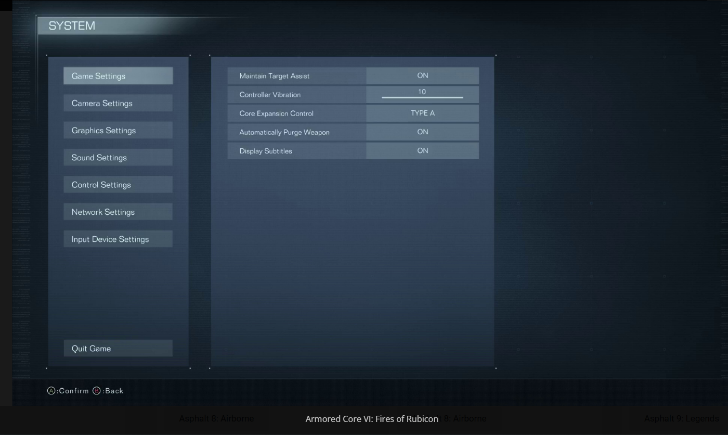
\includegraphics[width=0.8\textwidth]{settingsMenu.png}
    \caption{Settings Menu mit Ankerpunkten}
\end{figure}

Das gleiche Layout wurde in \FF auch implementiert, allerdings im Stil aller anderen UI-Elemente und beschränkt sich auf die Einstellungen, die programmiertechnisch bereits implementiert sind. Das Einstellungen Menu beinhaltet Audio Slider, welche Gesamtlautstärke, Musiklautstärke und Soundeffekte regulieren. Zusätzlich gibt es noch QOL (Quality of Life) Einstellungen, wie der \quoted{Show Screen Shake} Effekt bei einem Revolverschuss und eine Auswahl mit welchem Fenster das Spiel gestartet werden soll.

\begin{figure}[H]
    \centering
    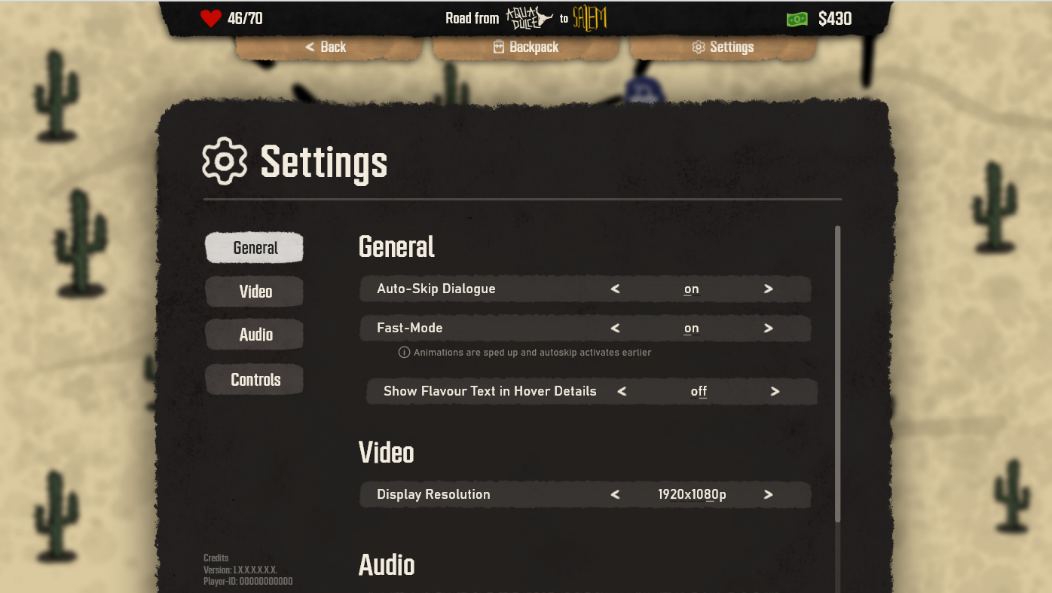
\includegraphics[width=0.8\textwidth]{settingsMockup.png}
    \caption{Settings Menu Mock-Up}
\end{figure}

\section{Bullet Designs}

Für ein Kartenspiel sei es nicht gewöhnlich, dass die Spielkarten, Kugeln sind und überhaupt, dass diese Karten in einen Revolver geladen werden. Das muss alles beim Entwerfen der Spielkarten von \FF berücksichtigt und im Hinterkopf behalten werden. Da \FF ein Setting im wilden Westen hat, wurde sich von alten Spielkarten aus dem wilden Westen Inspiration genommen. Im Laufe der Diplomarbeit wurde ein Guidelines Dokument erstellt, welches diese Inspiration erfasst. Beispielsweise zeigt folgende Collage an Bildern eine Idee, wie die Bullets in \FF gestaltet wurden.

\begin{figure}[H]
    \centering
    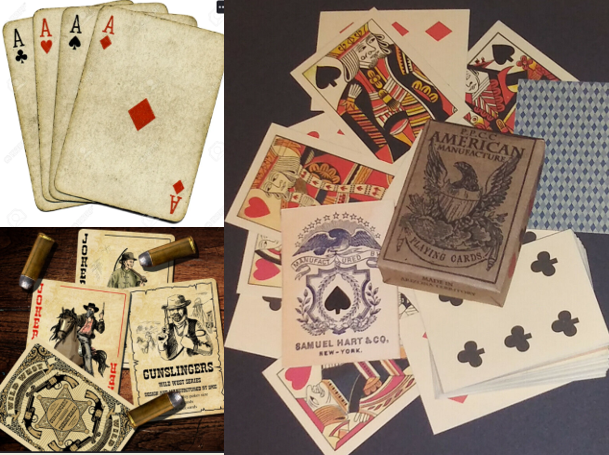
\includegraphics[width=0.8\textwidth]{bulletMoodboard.png}
    \caption{Moodboard Ausschnitt der Bullet Guidelines}
\end{figure}

Spielkarten weisen oft die Symbole \quoted{Pik} und \quoted{Karo} auf. Diese gehören zu den vier Farbsymbolen, die in Kartenspielen vorkommen können. In Kartenspielen werden diese Symbole verwendet, um die verschiedenen Karten zu kategorisieren und einzuteilen. Diese Symbole hatten damals bei der Entwicklungsphase von \FF noch eine Bedeutung. Es waren verschiedene Kategorien an Karten geplant, wurde jedoch die Bedeutung der Symbole aufgrund dem Game Design ausgelassen. Die Bullets weisen verhältnismäßig große abgerundete Kanten auf, um den Comic Stil des Spiels zu betonen. Daher wurden auch alle Bullets in einem Comic Stil gezeichnet. Das bedeutet, dass schwarze Outlines auf dem Design der Bullet an sich selbst sind, und die Bullet Designs hauptsächlich simpel gehalten sind. Letztendlich wurde sich für folgendes Design entschieden, als Vorlage für die nachkommenden Karten.

\begin{figure}[H]
    \centering
    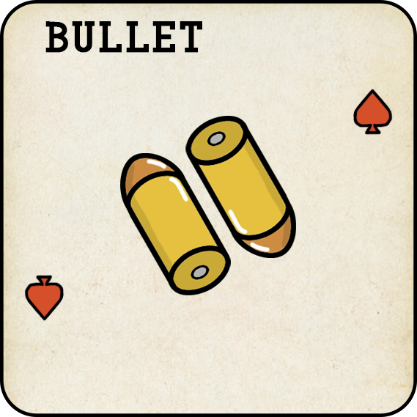
\includegraphics[width=0.4\textwidth]{bullet.png}
    \caption{Artwork der normalen Bullet}
\end{figure}

\begin{figure}[H]
    \centering
    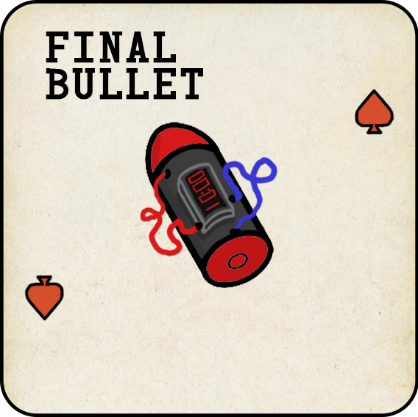
\includegraphics[width=0.4\textwidth]{finalBullet.png}
    \caption{Artwork der Final Bullet}
\end{figure}

\subsection{Bullet Photoshop Template}

Für ein Kartenspiel ist es üblich, dass dies hunderte, wenn nicht sogar tausende von Karten beinhalten. Diese zu designen, hat einen extrem hohen Zeitaufwand. Daher ist es besonders wichtig, einen guten Workflow zu haben und dafür ist ein Template essenziell. Einerseits wurde sich eine sinnvolle Ordnerstruktur für die hunderten Designs der Karten überlegt, welche dabei hilft, Ordnung zu halten, um schnell auf Bullets zugreifen zu können und um diese zu exportieren. Das Photoshop Template verfügt über mehrere Ordner, welche die Bereiche einer Karte zuständig sind. Beispielweise sind alle Texte, die auf einer Karte vorkommen, in dem grünen Ordner \quoted{Card Name} oder sind mit der Farbe Grün gekennzeichnet. Der Frame beziehungsweise die Form der Karte wurde mittels einer Quadrat Form mit abgerundeten Ecken erstellt. Diese Sorgt dafür, dass man nur innerhalb des Rahmens beziehungsweise der Karte zeichnen kann, und nicht aus Versehen rauszeichnet. Für den Namen der Bullets wurde eine Schriftart ausgewählt, welche einen rustikalen westlichen Touch hat. Serifen passen dazu besonders gut, da Serifen hauptsächlich in alten Schriftfamilien vorkommen und auch damals schon im wilden Westen verwendet wurden. Letztendlich wurde sich für die Schriftart
\quoted{Card Characters} entschieden, welche kostenlos und lizenzfrei im Internet zu finden ist, wie auf der Seite \url{https://www.fonts4free.net/}. Wenn Zeichen zu nah aneinander liegen, können Texte aus weiterer Entfernung oder niedriger Auflösung schwerer lesbar sein. Da die Spielkarten – wenn sie in der Hand während eines Kampfes sind – relativ klein sind, musste der Zeichenabstand als auch der Zeilenabstand auf die Größe der Karten angepasst werden, damit die Texte lesbarer sind. Für das Erstellen der meisten Bullets, wurden in dem Template die Ordner Frame, Symbols und Background nicht geändert. Einzelne Karten mit Besonderheiten, wie beispielsweise besonderen Effekten oder Karten, die erst spät im Spiel freigeschaltet werden können, erhalten zum Beispiel einen anderen Hintergrund, damit diese sich von den anderen Bullets abheben.

\vfill
\pagebreak

\begin{figure}[H]
    \centering
    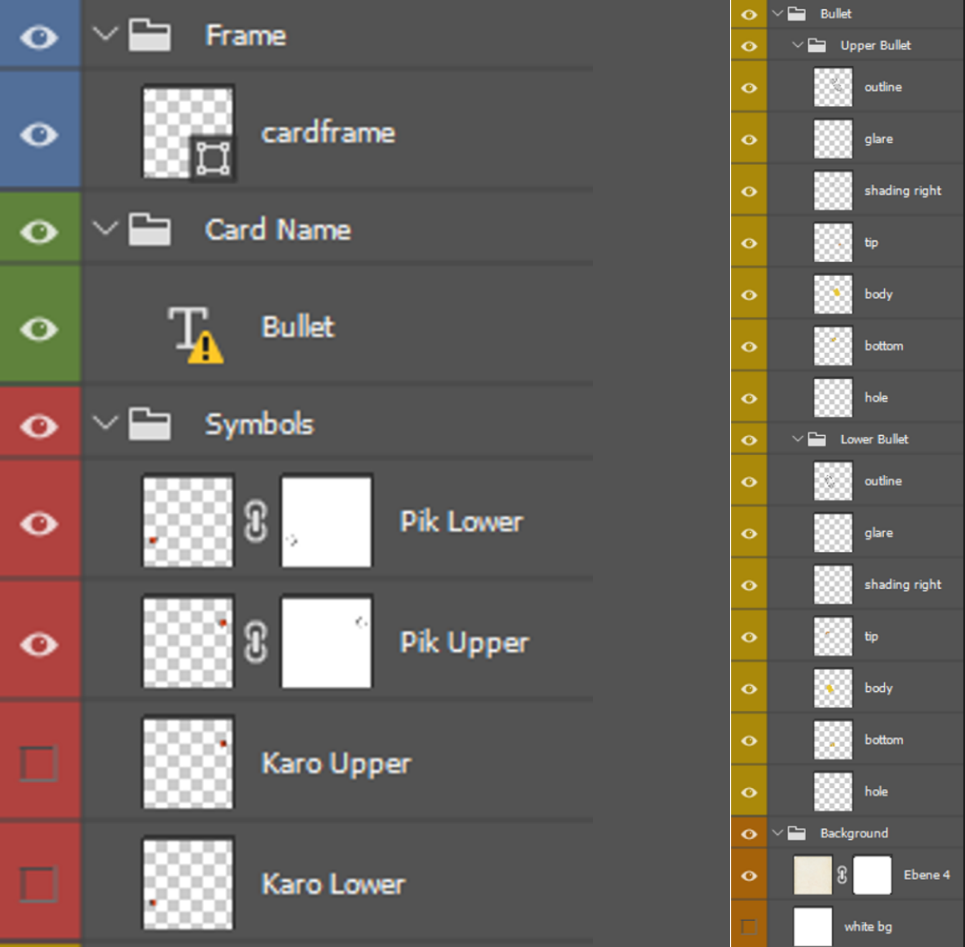
\includegraphics[width=0.6\textwidth]{bulletTemplate.png}
    \caption{Ebenen Struktur der Bullet Template}
\end{figure}

\subsection{Designvorgang einer Bullet}

Wenn für eine neue Karte nur die Farbe oder die Textur der Bullet geändert werden muss, erfolgt das mit dem Template sehr schnell. Es wird im Ordner \quoted{Bullet} die Ebene \quoted{Body} ausgewählt – zuständig für den Körper der Bullet Grafik – und ändert den Farbton der Bullet. Entweder mit dem Tastenkürzel
\quoted{STRG+U} oder über manuelle Suche das Fenster
\quoted{Farbton/Sättigung öffnen} geöffnet, worin mit einem Regler der Farbton geändert werden kann. Abschließend wird noch der Name der Karte
im \quoted{Card Name} Ordner geändert.

\begin{figure}[H]
    \centering
    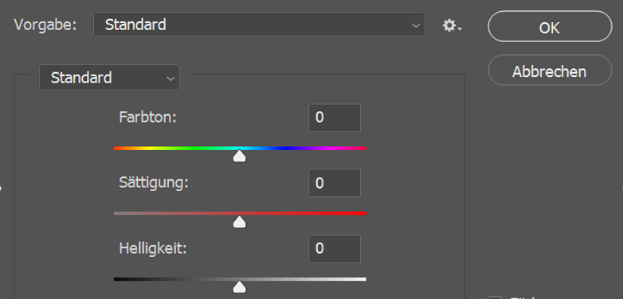
\includegraphics[width=0.6\textwidth]{farbtonRegler.png}
    \caption{Farbton/Sättigung Regler in Photoshop}
\end{figure}

Jedoch ist nicht jede Bullet einfach zu designen. Beispielsweise ist die \quoted{Eclipse Bullet} bei weitem komplizierter zu erstellen als eine andere Bullet, bei der sich mehr oder weniger nur die Farbe ändert. Eine Eclipse ist im deutschen übersetzt eine Sonnenfinsternis. Das Ziel war es, eine Bullet zu erstellen, die wie eine Sonnenfinsternis aussieht.  Als erstes wird eine Kopie des Templates in einem neuen Ordner
\quoted{Eclipse Bullet} erstellt. Danach wird ein passender Hintergrund für diese Karte ausgesucht. Um eine Sonnenfinsternis zu imitieren, muss die Karte Schwarz sein. Mit den Sternen im Hintergrund der Karte wird noch einmal betont, dass der Hintergrund das Weltall repräsentieren soll. Da diese Bullet einen besonderen Effekt haben wird, ist es gerechtfertigt, dass diese einen einzigartigen Hintergrund bekommt und somit von den anderen Karten hervorgehoben wird und als etwas besonderes erscheint. Für die Bullet an sich selbst, wurde zuerst eine schwarze Silhouette der Bullet erstellt, indem die
\quoted{Body}
Ebene ausgewählt wird und schwarz angemalt wird. Daraufhin wird eine Kopie dieser Ebene erstellt, welche direkt darüber liegt. Diese Ebene bekommt einen orangenen direktionalen Schlagschatten, welches über das Fülloptionen Menü in Photoshop und einer Ebenenmaske mit einem Verlauf von Schwarz auf Weiß erfolgt. Das bedeutet, dass der Schlagschatten an einem Ende der Bullet abnimmt, wie auf der zweiten Abbildung zu sehen ist. Im dritten Schritt wird ein innerer Schatten der Bullet hinzugefügt, was auch über die Fülloptionen mit der Funktion
\quoted{Innerer Schatten}
funktioniert. Das sorgt für einen realistischeren Glow Effekt auf der Bullet. Im letzten Schritt wird ein Linseneffekt eingebaut, welcher die Sonne, die hinter der Bullet ist, repräsentiert. In Photoshop kann unter dem Reiter
\quoted{Filter} und \quoted{Renderfilter} einBlendenfleck hinzugefügt werden. Dort sind verschiedene Objektivarten auszuwählen, die verschiedene Blendenflecke erzeugen.
Die Option \quoted{35mm}
sieht am ehesten aus wie eine Sonne. Dieser Linseneffekt wurde noch an den Rand der Bullet platziert, was es so wirken lässt, als würde eine Sonne hinter der Bullet leuchten. Anschließend wird die Bullet in der Auflösung 500x500 Pixel als PNG (Portable Network Graphics) exportiert, damit die abgerundeten Ecken erhalten bleiben.

\begin{figure}[H]
    \centering
    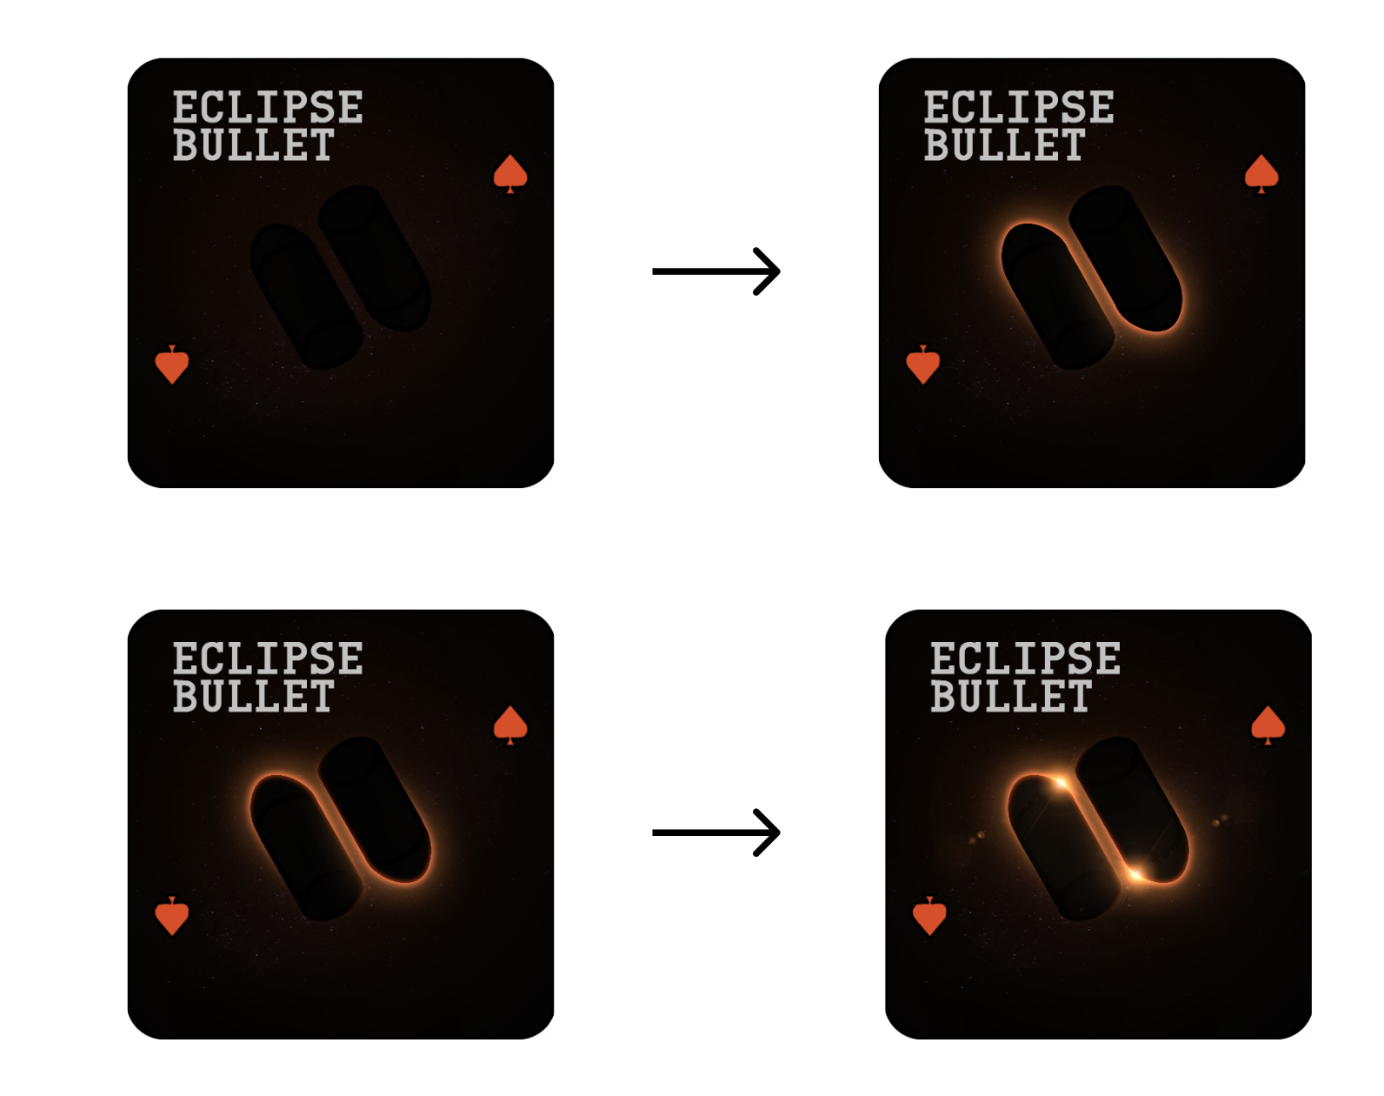
\includegraphics[width=1.0\textwidth]{eclipseBullet.png}
    \caption{Aufbau der Eclipse Bullet in vier Schritten}
\end{figure}

\section{Artstyle}\label{sec:artstyle}

\renewcommand{\kapitelautor}{Autor: Philip Jankovic}

\FF in game visuals sind handgezeichnet und oft statisch. Beim Zeichnen wurde zuerst eine "Reference" gesucht.


\subsection{References}\label{subsec:references}
References beim Zeichnen sind Bilder oder andere Artworks an denen sich orientiert wird. Vorallem am Anfang ist das
Arbeiten mit References fast ein Muss, da das einfache Vorstellen der Zeichnung im Kopf und das anschließende Zeichnen davon höchst anspruchsvoll ist.
Die Perspektive, Kleidung und Körperposen können von der Reference inspiriert werden.
Jedoch wird versucht die Reference nicht 100\% abzuzeichnen, sondern auch den eigenen Stil hinzufügen. \zit{referance}


Für \FF wurden References von "Pinterest", jedoch auch Inspirationen aus diversen Filmen und anderen Medien gesucht. \zit{pinterest}


Ein Beispiel für die Nutzung verschiedenster References ist der Manga \quoted{JOJO's Bizarre Adventure} von Hirohiko Araki\zitbuch{jojo},
welcher auch eine Inspiration für einige Teile von \FF ist. Nicht nur im Bezug auf die Zeichnungen, sondern auch auf die von dem Autor benützen Krativfindungsmethoden.
Mehr dazu kann in dem Kapitel \ref{sec:methoden} gelesen werden.
Araki verwendet eine große Auswahl als References für seine Zeichnungen, vorallem aus der Welt
der Fashion, was auch in seinem Artstyle zu sehen ist.


\FF bezieht auch ein paar References von "JOJO's Bizarre Adventure", jedoch ist die Auswahl der benützten References groß und abwechslungsreich.
Auch eigene selbst fotografierte Reference-Bilder wurden verwendet für \zB den Main-Charackter des Spieles.

\begin{figure}[H]
    \centering
    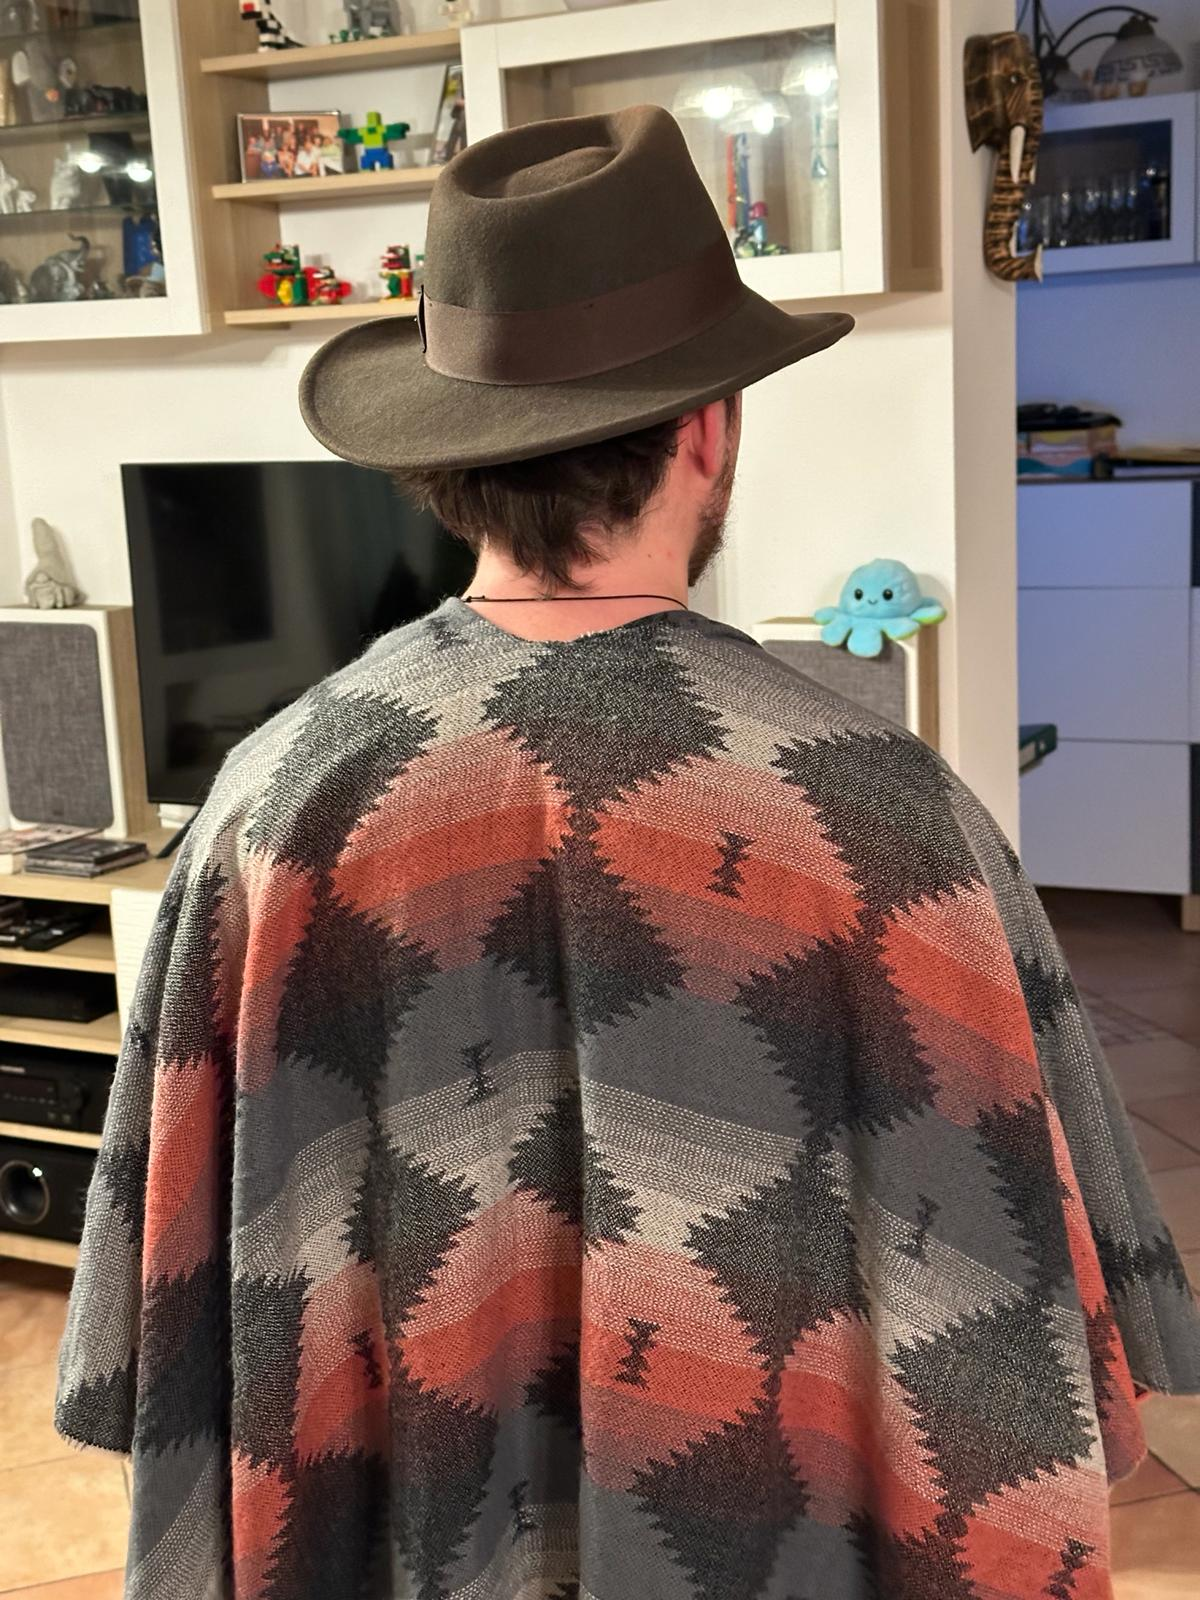
\includegraphics[width=0.4\textwidth]{mainchar.jpg}
    \caption{Beispiel: Reference von der Spieler-Zeichnung}
\end{figure}

Bei dem Nutzen einer Reference muss jedoch darauf geachtet werden, das Bild nicht nur abzuzeichnen. Je nach Zeichenstil
oder wie stilisiert ein Zeichenstil ist, besteht eine Gefahr, ein Bild nur abzuzeichnen, anstatt es als Reference zu verwenden.
Das Bewahrens eines eigenen Zeichenstiles ist dabei besonders wichtig.


\subsection{Artstyle von \FF}\label{subsec:artsytle}

Der Artstyle von \FF ist im Comic-stil gehalten, mit groben, Bleistift Outlines und Coloring auf der Ebene darunter.
Coloring wird mit einem Farbpinsel auf 100\% Fluss gemacht, damit die Kanten schön hart sind und es sich besser von dem Hintergrund abheben.
Auch wenn die Zeichnungen selber nicht realistisch gezeichnet sind, halten sie sich an realistische Posen und Propertionen, sind also nicht wirklich stilisiert.
Das Spiel nimmt sich dadurch nicht zu ernst, passt aber gut zu dem rauen Wild-West Setting und schlägt für den Betrachter trotz all dieser komischen Bullets
einen Anker in der Realität.

\begin{figure}[H]
    \centering
    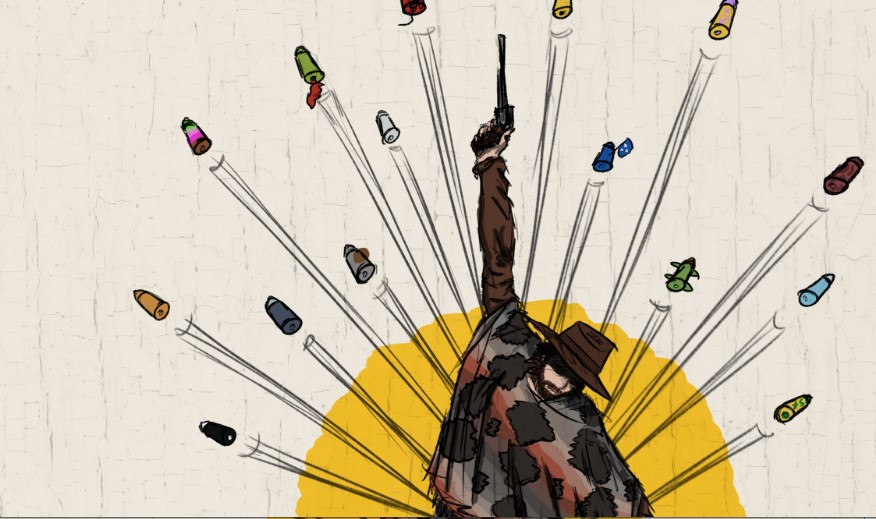
\includegraphics[width=0.8\textwidth]{artstylepic.jpg}
    \caption{Beispiel: Artstyle von \FF}
\end{figure}

\begin{figure}[H]
    \centering
    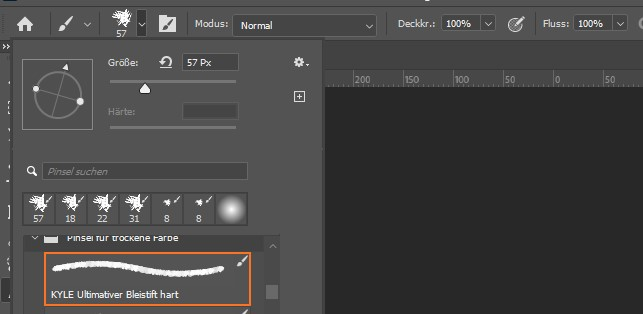
\includegraphics[width=0.8\textwidth]{outline.jpg}
    \caption{Beispiel: Verwendeter Ouline Brush}
\end{figure}

\begin{figure}[H]
    \centering
    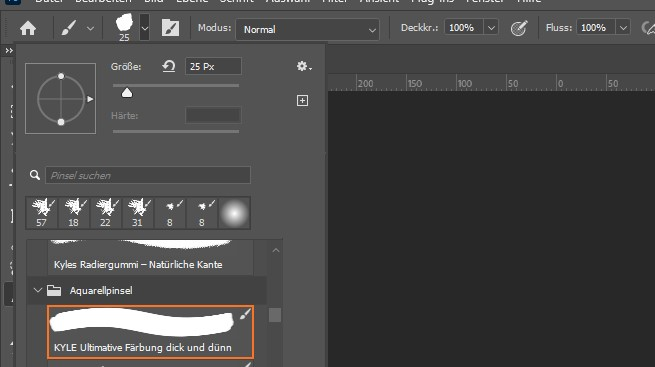
\includegraphics[width=0.8\textwidth]{color.jpg}
    \caption{Beispiel: Verwendeter Colering und Shading Brush}
\end{figure}


Um den Zeichnungen mehr Tiefe zu geben wird über der Color-Ebene eine Muliplate-Ebene auf 50\% Oppacity verwendet um Schatten
darzustellen. Geshaded wird mit dem selben Pinsel mit welchem Gecolored wird. Das Shading bleibt bei diesem einen grauen ton,
härtere shadows werden durch "Crosshatching" mit dem Outline-Bleistift gemacht.\zit{crosshatching}

\begin{figure}[H]
    \centering
    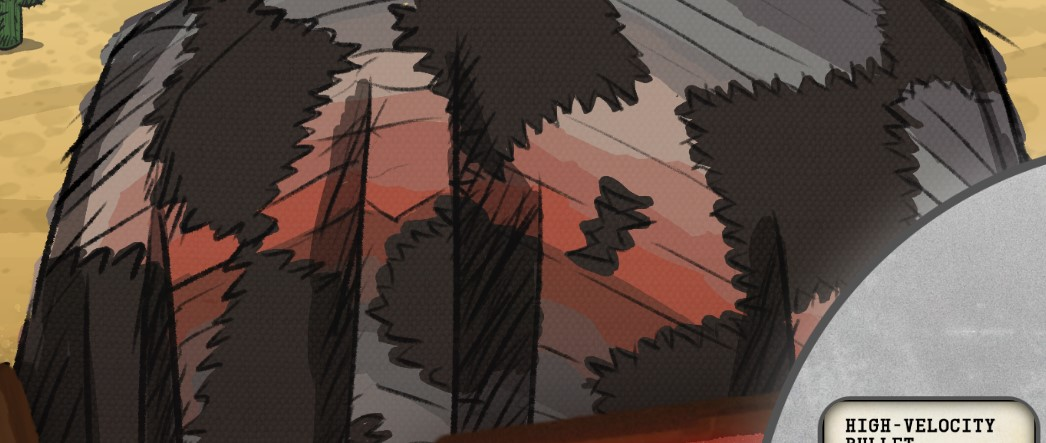
\includegraphics[width=0.4\textwidth]{crossha.jpg}
    \caption{Beispiel: Crosshatching in \FF}
\end{figure}

\renewcommand{\kapitelautor}{}
